%\documentclass[a4paper, 12pt, notitlepage]{report}
\documentclass[11pt,a4paper]{article}
\usepackage[T1]{fontenc}
\usepackage{textcomp}

\usepackage[utf8]{inputenc}
\usepackage[english]{babel}
\usepackage{verbatim}
\usepackage{listings}

\usepackage{hyperref}
\usepackage{etoc}

\usepackage{float}
\usepackage{amsmath}
\usepackage{amsfonts}
\usepackage{mathtools}

\usepackage{fancyvrb}
\usepackage{xcolor}

\usepackage{graphicx} % graphics package

\setlength{\parindent}{5pt}
\usepackage[margin=0.5cm]{geometry} 
\geometry{
    a4paper,
    top=20mm,
    bottom =20mm,
    left=25mm,
    right=25mm
    }

%%%%%%%%%%%%%%%%%%%%%%%%%%%%%%%%%%%%%%%%%%%%%%%%%%%%%%%%%%
% Paquetes agregados por mi
\usepackage[font=small,labelfont=bf,hypcap=false]{caption} % Required for specifying captions to tables and figures
\usepackage{titlesec}
\setcounter{secnumdepth}{4}
\usepackage{tcolorbox}
\tcbuselibrary{theorems}
\usepackage{subfigure}

\usepackage[shortlabels]{enumitem}
\usepackage{multirow} 
\usepackage{colortbl}
\setlist[itemize]{label=\textbullet}

\usepackage{rotating}
\usepackage{pdflscape}
\usepackage{lscape}

\usepackage[maxnames=1,style=numeric,sorting=none]{biblatex}
\addbibresource{ref.bib}
\usepackage{csquotes}

\usepackage[yyyymmdd]{datetime}
\usepackage{ulem}

\usepackage[export]{adjustbox}

\usepackage{tikz}
\usetikzlibrary{shapes.geometric, arrows.meta,arrows}
\tikzset{basic/.style={draw,fill=none,
                       text badly centered,minimum width=3em}}
\tikzset{input/.style={basic,circle,minimum width=3.5em}}
\tikzset{weights/.style={basic,rectangle,minimum width=2em}}
\tikzset{functions/.style={basic,circle, minimum width=4em}}
\tikzset{bias/.style={basic,circle, minimum width=4em}}
\tikzset{myarrow/.style=-{Stealth[length=3mm, width=2mm]}}

\newcommand{\addaxes}{\draw (0em,1em) -- (0em,-1em)
                            (-1em,0em) -- (1em,0em);}
\newcommand{\relu}{\draw[line width=1.5pt] (-1em,0) -- (0,0)
                                (0,0) -- (0.75em,0.75em);}
\newcommand{\stepfunc}{\draw[line width=1.5pt] (0.65em,0.65em) -- (0,0.65em) 
                                    -- (0,-0.65em) -- (-0.65em,-0.65em);}

\newcommand{\MYhref}[3][blue]{\href{#2}{\color{#1}{#3}}}%

% Input layer neurons'number
\newcommand{\inputnum}{3} 
 
% Hidden layer neurons'number
\newcommand{\hiddennum}{5}  
 
% Output layer neurons'number
\newcommand{\outputnum}{1} 

\usepackage{tikz-3dplot}
\usetikzlibrary{3d}
\definecolor{dgreen}{RGB}{63,127,0}
\definecolor{dred}{RGB}{144,14,3}
\tdplotsetmaincoords{60}{50}

\usepackage{algorithm}
\usepackage{algpseudocode}

\usepackage{amssymb}
\usepackage{bm}
\usetikzlibrary{arrows.meta}
\usetikzlibrary{decorations.pathreplacing}

\usepackage{pgfplots}

\usepackage{svg}
%%%%%%%%%%%%%%%%%%%%%%%%%%%%%%%%%%%%%%%%%%%%%%%%%%%%%%%%%%


\renewcommand*\contentsname{Indice}

% \unisalento command
\newcommand{\unisalento}{\href{http://www.unisalento.it}{\textbf{\emph{Università del Salento}}}}

% colors for code snippets
\definecolor{codegreen}{rgb}{0,0.7,0.5}
\definecolor{codegray}{rgb}{0.5,0.5,0.5}
\definecolor{codeblue}{rgb}{0,0.5,0.82}
\definecolor{backcolour}{rgb}{0.95,0.95,0.95}

\lstdefinestyle{mystyle}{
    backgroundcolor=\color{backcolour},   
    commentstyle=\color{codegreen},
    keywordstyle=\color{orange},
    numberstyle=\tiny\color{codegray},
    stringstyle=\color{codeblue},
    basicstyle=\ttfamily\footnotesize,
    breakatwhitespace=false,         
    breaklines=true,                 
    captionpos=b,                    
    keepspaces=true,                 
    numbers=left,                    
    numbersep=5pt,                  
    showspaces=false,                
    showstringspaces=false,
    showtabs=false,                  
    tabsize=2
}

\lstset{style=mystyle}
\title{
    
\includegraphics[scale=1]{Tesis/media/logo-utn-ba.png}
    
    \vspace{1cm}
    {\Huge{\textbf{Universidad Tecnológica Nacional}}}
    
    \normalfont{Curso de grado}
    \par\noindent\rule{\textwidth}{0.4pt}
    
    \vspace{0.3cm}

    \par \Large{\textbf{Sistema de navegación inteligente acelerado por hardware}}
    
    \vspace{1.0cm}

    \begin{flushleft} \large
    
    \textsc{ \textbf{Director:} Ing. Silvio Abel Tapino}\\
    \hfill \break
    \textsc{ \textbf{Tutor:} Ing. Alejandro Furfaro}\\
    \hfill \break
    \textsc{ \textbf{Co-tutor:} Ing. Luciano Ferreyro}\\
    \hfill \break
    \textsc{ \textbf{Tutor por la cátedra:} Dr. Ing. Matias Hampel}\\
    \hfill \break
    \textsc{ \textbf{Tutor por la cátedra:} Ing. Maria Alejandra Gutierrez}\\
    \hfill \break
    \textsc{ \textbf{Autor:} Martín Fuschetto} % Your name
    \emph{(mfuschetto@frba.utn.edu.ar)}\\[1cm]
    
    \end{flushleft}

    \vspace{5cm}
    
    \par\noindent\rule{\textwidth}{0.4pt}
    \vspace{0.1cm}
    
    \small{AÑO ACADÉMICO 2021/2022}
    \thispagestyle{empty}
    }
    
\author{} % lasciare vuoto
\date{}   % lasciare vuoto

\hypersetup{hidelinks}

\begin{document}
    % frontispiece creation
    \maketitle

    % blank page
    \mbox{}
    \thispagestyle{empty}
    
    % index creation
    \newpage
    \hypersetup{hidelinks}
    \tableofcontents
    \thispagestyle{empty}
    
    % Chapter: "Credits"
    \newpage
    \hypersetup{hidelinks}
    \section{AGRADECIMIENTOS}

... (TERMINAR)
    
    % Introduccion
    \newpage
    \hypersetup{hidelinks}
    \section{INTRODUCCIÓN}

Tradicionalmente la robótica estaba centrada en sectores industriales manufactureros orientados a la producción masiva. A mediados de los 60's se introducen robots manipuladores en distintos tipos de industrias. Típicamente los robots desarrollaban tareas repetitivas, el cual exigía tomar algunas piezas y reubicarlas en otra área a la cual el robot manipulador sea capaz de llegar con la máxima extensión de su articulación lo cual resultaba en un problema. Una solución a este problema fué desarrollar un vehículo móvil sobre rieles y así es como a mediado de los 80's aparecieron los primeros vehículos guiados automáticamente (AGV's).\par
Fuera del entorno industrial, en donde se imposibilitaba estructurar el entorno, se les doto a los robots un mayor grado de inteligencia y capacidad para poder desenvolverse.\par

Uno de los desafíos mas grandes en la aplicación de robots es la navegación en entornos desconocidos abarrotados de obstáculos. La navegación se vuelve aun mas compleja cuando se desconoce la ubicación de estos a priori. Se introdujo así entonces el concepto de conjunto difuso (Fuzzy Set) bajo el que reside la idea de que los elementos sobre los que se construye el pensamiento humano no son números sino etiquetas lingüísticas. \par

La lógica difusa se ha utilizado en el diseño de múltiples posibles soluciones en donde se han creado distintos sistemas de control de navegación orientados a robots para que estos puedan llegar a destino evitando obstáculos en su camino.\par 
A lo largo de los años se han desarrollado algunos enfoques distintos, uno muy particular en el cual la navegación se divide en dos partes. La primera compuesta en comportamientos básicos tales como: lograr metas, evitación de obstáculos y seguimiento de muros. La segunda, una capa de supervisión responsable de la selección de las acciones (elección de comportamientos según el contexto). \par

El principal aporte de mi proyecto de investigación es realizar un sistema de control neuro-difuso nuevo que solo va a necesitar un controlador difuso pero que además, va a estar dividido en dos partes: \par
La primera (difuso) con comportamientos básicos: lograr metas, evitación de obstáculos, etc. A partir de ahora llamado \textbf{"Modulo de sistema de control difuso"}. \par
La segunda de supervisión (neuronal) en donde se va a seleccionar, arbitrar o fusionar comportamientos de la lista de estos en función de la salida del sistema neural convolucional el cual tendrá la capacidad de, a través de una cámara, poder reconocer el obstáculo a evadir y en función de la ubicación y dimensión de este decidir un comportamiento difuso. A partir de ahora llamado \textbf{"Modulo de procesamiento de imágenes"}. \par
Siempre buscando con esta idea que la toma de decisión se parezca un poco mas a la del ser humano, elegir un rumbo en función de lo que el robot ve y reconoce, ya que desde mi punto de vista es antinatural la elección de trayectoria solo en función de la ubicación del obstáculo y el target (destino), hay que tener en cuenta que nosotros, al encontrar un obstáculo que nos evita el paso también evaluamos el trayecto a seguir en función de las dimensiones del obstáculo y del largo del trayecto a recorrer. Por ejemplo al eludir un obstáculo muchas veces evaluamos si eludir por la izquierda o por la derecha es mas conveniente en función del largo de ambos caminos.\par

La detección de objetos es una tarea de suma importancia para la conducción autónoma, junto con esta tarea viene aparejada la responsabilidades de garantizar la precisión a la hora de detectar estos objetos y a su vez, de suma importancia, inferirlo en tiempo real para garantizar el adecuado control del móvil. 
Para satisfacer todas estas necesidades se propuso implementar una SqueezeDet, una red neuronal totalmente convolucional para la detección de objetos caracterizada por su precisión, tamaño, velocidad y consumo de energía. \par

La investigación fue llevada a cabo en el marco de la materia Proyecto Final de la carrera de Ingeniería Electrónica de la Universidad Tecnológica Nacional (Regional Buenos Aires), y fue auspiciada por el Laboratorio de Procesamiento Digital (DPLAB) del Departamento de Electrónica de dicha facultad regional. La investigación realizada y el diseño final quedaron
a disposición del DPLAB como base para futuros trabajos de investigación. \par

Se inicia este trabajo en un capitulo en donde se presenta el marco teorico del proyecto. ... (TERMINAR) \par



    % MArco teorico
    \newpage
    \hypersetup{hidelinks}
    \section{MARCO TEÓRICO}

% Redes Neuronales Convolucionales
\subsection{Redes Neuronales Convolucionales}

\subsubsection{Introducción}

Sin duda alguna en la ultima década las redes neuronales convolucionales se popularizaron en gran medida. Todo comenzó con una nueva forma de computación inspirada en modelos biológicos, los cuales consisten en sistemas con un gran numero de procesos interconectados funcionando en paralelo los cuales procesan información y tienen la capacidad de aprender a través de la experiencia.\par
La detección de objetos en imágenes es una tarea de suma importancia a la hora de realizar un sistema de navegación autónomo, las redes neuronales vienen a resolver el problema.\par
Dentro de las las redes neuronales hay distintos tipos y una de ellas son las redes neuronales convolucionales (CNN) las cuales están inspiradas en las neuronas de la corteza visual primaria del cerebro. Estos tipos de redes neuronales pueden dotar a los robots de visión y es por eso que vienen a resolver el problema.\par
De esta forma esta sección de la tesis se enfocara en aportar un marco teórico de las redes neuronales convolucionales.\par

\subsubsection{El perceptrón}

En 1957 Frank Rosenblatt comenzó el desarrollo de una red neuronal a la que denomino ''El perceptrón'' fue tal su aporte que hoy en día se lo utiliza para reconocer patrones. Este modelo fue capaz de generalizar, es decir que luego un aprendizaje de ciertos patrones, y a pesar de sus limitaciones (era incapaz de resolver la OR exclusiva y en general incapaz de clasificar clases no separables linealmente) era capaz de reconocer patrones que jamas se le hayan presentado.
La entrada de la función de activación se calcula como la suma ponderada de todas las entradas del perceptrón más un valor de bias.\par

\begin{figure}[!h]
\centering
    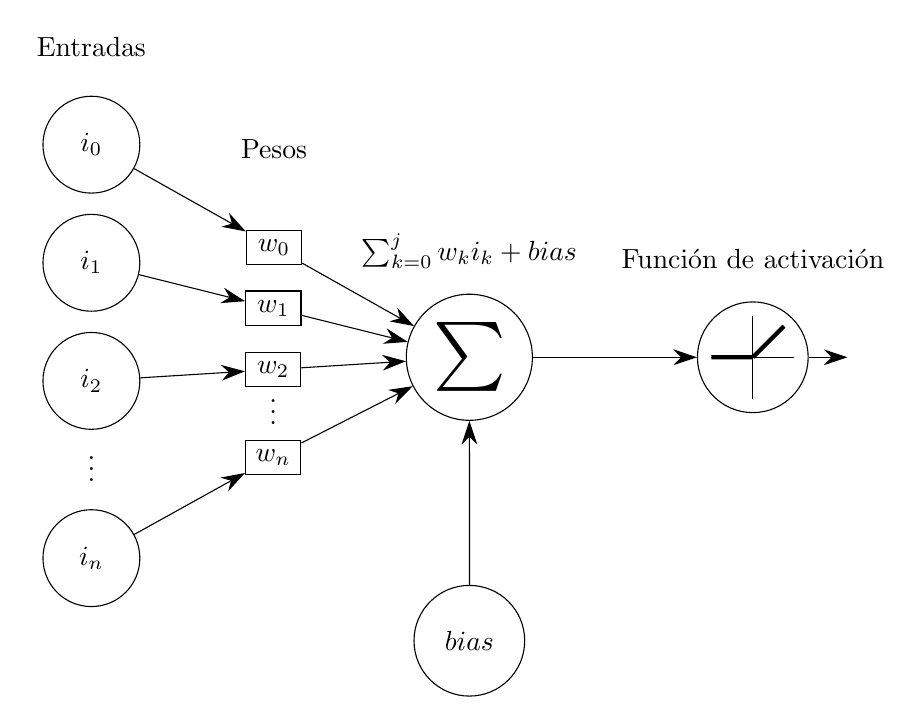
\begin{tikzpicture}[scale=1.2]
    % Draw input nodes
    \foreach \h [count=\hi ] in {$i_2$,$i_1$,$i_0$}{%
          \node[input] (f\hi) at (0,\hi*1.25cm-1.5 cm) {\h};
        }
    % Dot dot dot ... x_n
    \node[below=0.62cm] (idots) at (f1) {\vdots};
    \node[input, below=0.62cm] (last_input) at (idots) {$i_n$};
    % Draw summation node
    \node[functions] (sum) at (4,0) {\Huge$\sum$};
    \node[above=1cm] at (sum) {$\sum_{k=0}^j w_ki_k + bias$};
    % Draw bias node
    \node[bias] (biass) at (4,-3) {$bias$};
    \draw[myarrow] (biass) -- (sum);
    % Draw edges from input nodes to summation node
    \foreach \h [count=\hi ] in {$w_2$,$w_1$,$w_0$}{%
          \path (f\hi) -- node[weights] (w\hi) {\h} (sum);
          \draw[myarrow] (f\hi) -- (w\hi);
          \draw[myarrow] (w\hi) -- (sum);}
    % Dot dot dot ... w_n
    \node[below=0.05cm] (wdots) at (w1) {\vdots};
    \node[weights, below=0.45cm] (last_weight) at (wdots) {$w_n$};
    % Add edges for last node and last weight etc
    \path[draw,myarrow] (last_input) -- (last_weight);
    \path[draw,myarrow] (last_weight) -- (sum);
    % Draw node for activation function
    \node[functions] (activation) at (7,0) {};
    % Place activation function in its node
    \begin{scope}[xshift=7cm,scale=1.25]
        \addaxes
        % flexible selection of activation function
        \relu
        % \stepfunc
    \end{scope}
    % Connect sum to relu
    \draw[myarrow] (sum) -- (activation);
    \draw[myarrow] (activation) -- ++(1,0);
    % Labels
    \node[above=1cm]  at (f3) {Entradas};
    \node[above=1cm] at (w3) {Pesos};
    \node[above=1cm] at (activation) {Función de activación};
    \end{tikzpicture} 
\captionof{figure}{El perceptrón}
\label{fig:elperceptron}
\end{figure}

\subsubsection{¿Que es una red neuronal?}

Una red neuronal es un grupo interconecto de distintos elementos procesadores simples que operan en paralelo, cuya función se determina a partir de distintas características de la red, su estructura, la fuerza o pesos en las conexiones y el procesamiento realizado en cada nodo.\par
Muchas veces se la define como un aproximador universal. El modelo conocido como perceptrón multicapa esta compuesto por ''k'' capas de neuronas que están interconectadas y cada salida de cada neurona es la suma ponderada de todas las salidas de las neuronas de la capa anterior mas un valor de bías (\autoref{fig:elperceptron}).

\begin{figure}[!h]
\centering
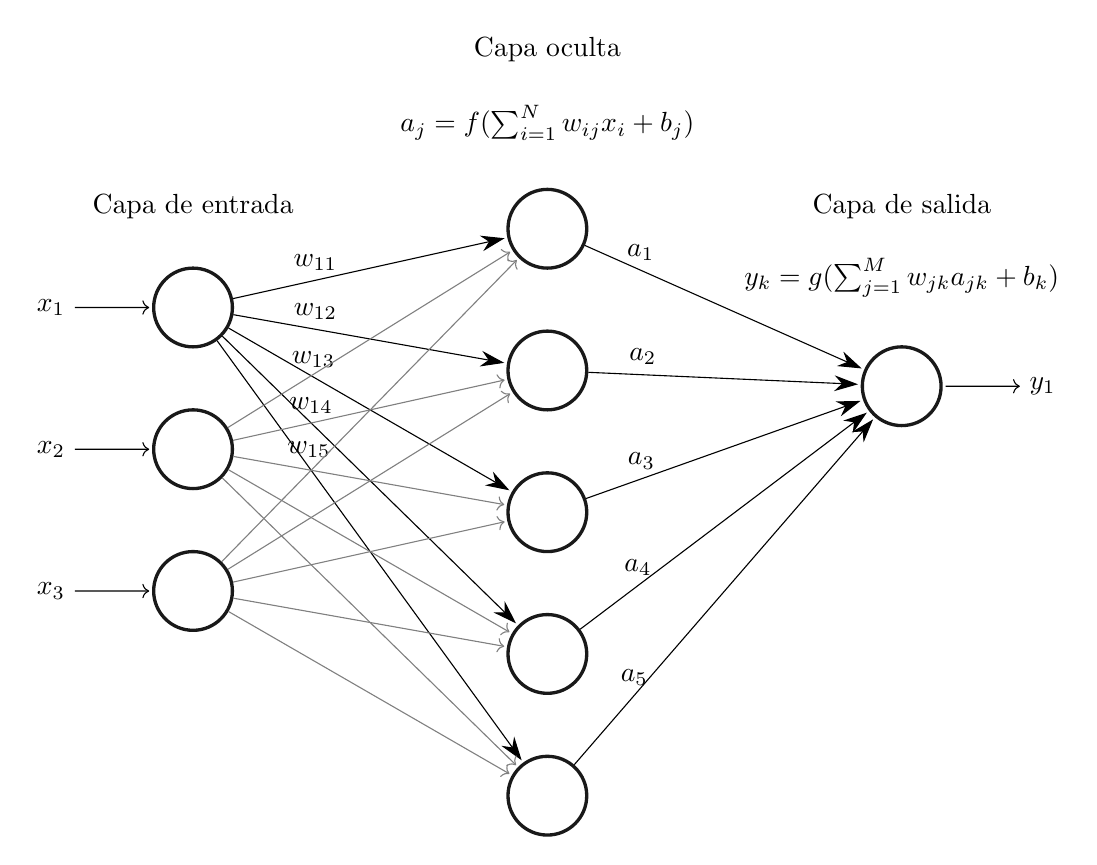
\begin{tikzpicture}[scale=1.5]
 
% Input Layer
\foreach \i in {1,...,\inputnum}
{
    \node[circle, 
        draw=black!90,
        very thick,
        minimum size = 10mm,
        fill=white!30] (Input-\i) at (-1.5,-\i*1.2) {};
}
\node[above=1cm] at (Input-1) {Capa de entrada}; % nombre de la capa
 
% Hidden Layer
\foreach \i in {1,...,\hiddennum}
{
    \node[circle, 
        draw=black!90,
        very thick,
        minimum size = 10mm,
        fill=white!50,
        yshift=(\hiddennum-\inputnum)*5 mm
    ] (Hidden-\i) at (1.5,-\i*1.2) {};
}
\node[above=2cm] at (Hidden-1) {Capa oculta}; % nombre de la capa
\node[above=1cm] at (Hidden-1) {$a_j = f(\sum_{i=1}^N w_{ij}x_i + b_j)$}; % nombre de la capa

% Output Layer
\foreach \i in {1,...,\outputnum}
{
    \node[circle, 
        draw=black!90,
        very thick,
        minimum size = 10mm,
        fill=white!50,
        yshift=(\outputnum-\inputnum)*5 mm
    ] (Output-\i) at (4.5,-\i*1.2) {};
}
\node[above=2cm] at (Output-1) {Capa de salida}; % nombre de la capa
\node[above=1cm] at (Output-1) {$y_{k} = g(\sum_{j=1}^M w_{jk}a_{jk} + b_k)$}; % nombre de la capa

% Connect neurons In-Hidden
\foreach \i in {1,...,\inputnum}
{
    \foreach \j in {1,...,\hiddennum}
    {
        \ifthenelse{ \i = 1 } 
        {\draw[->, shorten >=1pt,myarrow,black] (Input-\i) -- (Hidden-\j) node [pos=0.3,above] {$w_{\i\j}$};} 
        {\draw[->, shorten >=1pt, gray] (Input-\i) -- (Hidden-\j);}
    }
}
 
% Connect neurons Hidden-Out
\foreach \i in {1,...,\hiddennum}
{
    \foreach \j in {1,...,\outputnum}
    {
        %\draw[->, shorten >=1pt] (Hidden-\i) -- (Output-\j);
        \ifthenelse{ \j = 1 } 
        {\draw[->, shorten >=1pt,myarrow,black] (Hidden-\i) -- (Output-\j) node [pos=0.2,above] {$a_{\i}$};} 
        {\draw[->, shorten >=1pt, gray] (Hidden-\i) -- (Output-\j);}
    }
}
 
% Inputs
\foreach \i in {1,...,\inputnum}
{            
    \draw[<-, shorten <=1pt] (Input-\i) -- ++(-1,0) node[left]{$x_{\i}$};
}
 
% Outputs
\foreach \i in {1,...,\outputnum}
{            
    \draw[->, shorten <=1pt] (Output-\i) -- ++(1,0) node[right]{$y_{\i}$};
}
 
\end{tikzpicture} 
\captionof{figure}{Perceptrón multicapa}
\label{fig:elperceptronmulticapa}
\end{figure}

Debido a que la salida de una determinada neurona de la capa ''k'' se calcula utilizando todas las salidas de la neurona anterior se denomina capa de neuronas ''fully conected''.\par

\begin{itemize}
    \item Vector x: Entrada de la capa (conformado por las salidas de cada una de las neuronas de la capa anterior).
    \item n: Cantidad de neuronas de la capa anterior.
    \item Vector y: Vector de salidas.
    \item m: Cantidad de neuronas de la capa a calcular.
    \item Matriz w: Coeficientes de la capa ''fully connected''.
    \item Vector b: Bias de la capa ''fully connected''.
\end{itemize}

\[
   \begin{bmatrix} 
    w_{11} & \dots  & w_{1n} \\
    \vdots & \ddots & \vdots \\
    w_{m1} & \dots  & w_{mn} 
    \end{bmatrix}
    *
    \begin{bmatrix} 
    x_{1} \\
    \vdots \\
    x_{n} 
    \end{bmatrix}
    +
    \begin{bmatrix} 
    b_{1} \\
    \vdots \\
    b_{m} 
    \end{bmatrix}
    =
    \begin{bmatrix} 
    y_{1} \\
    \vdots \\
    y_{m} 
    \end{bmatrix}
    = 
    \begin{bmatrix} 
    a_{1} \\
    \vdots \\
    a_{m} 
    \end{bmatrix}
\]

\subsubsection{Capas convolucionales}

La principal diferencia de una red neuronal convolucional de cualquier otro red neuronal es que utiliza una operación llama ''convolución'' en algunas de sus capas en vez de utilizar la multiplicación de matrices. Esta operación recibe como entrada una imagen y luego le aplica un filtro (también llamado ''kernel'') y retorna otra imagen con las características de la imagen de entrada.\par
A continuación el proceso: \par

\begin{figure}[!h]
    \centering
    \begin{tikzpicture}

    % Simbolo de conv
    \begin{scope}[shift={(4,-0.3)},rotate=45, scale=0.5]
        \draw[-] (0,0,0) circle(1cm);
        \draw[-] (0,-1)--(0,1)--cycle;
        \draw[-] (-1,0)--(1,0)--cycle;
    \end{scope}
    
    % igual
    \begin{scope}[shift={(10.5,-0.5)},rotate=0, scale=0.35]
        \draw[-] (-1,1)--(1,1)--cycle;
        \draw[-] (-1,0)--(1,0)--cycle;
    \end{scope}
    
     % Matriz de entrada
    \begin{scope}[tdplot_main_coords,line join=miter,font=\sffamily, xshift=0, yshift=0cm]
        \pgfmathsetmacro{\xstretch}{1}
        \edef\Cols{white, white, white}
        \edef\LstCols{{"white", "white", "white"}}
        
        \foreach \Col [count=\X starting from 0,remember=\X as \LastX] in \Cols
        {  
            \foreach \XX in {1}
            {  
                \draw[thick,\Col] (\xstretch*\X+0.4*\XX-0.1,0,0) -- (\xstretch*\X+0.4*\XX,0,0);
                \begin{scope}[canvas is yz plane at x=\xstretch*\X+0.4*\XX]
                    \pgfmathtruncatemacro{\fullness}{120-20*\XX}
                    \draw[fill=\Col!\fullness] (-1,-1) rectangle (1,1);
                \end{scope}
            }
            %\node[anchor=west] at (\xstretch*\X,-2,-2){$x_\X$};
        }
        \node[anchor=west] at (\xstretch,-1.5,-1.5){$N_{iz}$};
        \node[anchor=west] at (\xstretch,1,-2.5){$N_{ix}$};
        \node[anchor=west] at (\xstretch,2.5,-1.5){$N_{iy}$};
        \node[anchor=west] at (\xstretch,-1,3){Matriz de entrada};
    \end{scope}
    % cuadraditos en la matriz de entrada
    \begin{scope}[tdplot_main_coords,line join=miter,font=\sffamily, xshift=-5, yshift=5, scale=0.2]
        \pgfmathsetmacro{\xstretch}{1}
        \edef\Cols{white, white, white}
        \edef\LstCols{{"white", "white", "white"}}
        
        \foreach \Col [count=\X starting from 0,remember=\X as \LastX] in \Cols
        {  
            \foreach \XX in {1}
            {  
                \draw[thick,\Col] (\xstretch*\X+0.4*\XX-0.1,0,0) -- (\xstretch*\X+0.4*\XX,0,0);
                \begin{scope}[canvas is yz plane at x=5*\xstretch*\X+0.4*\XX]
                    \pgfmathtruncatemacro{\fullness}{120-20*\XX}
                    \draw[fill=\Col!\fullness, draw=red] (-1,-1) rectangle (1,1);
                \end{scope}
            }
            %\node[anchor=west] at (\xstretch*\X,-2,-2){$x_\X$};
        }
    \end{scope}


    % Grupo de filtros
    \begin{scope}[tdplot_main_coords,line join=miter,font=\sffamily, xshift=5.5cm, yshift=0.2cm, scale=0.6]
        \pgfmathsetmacro{\xstretch}{1}
        \edef\Cols{red, green, blue}
        \edef\LstCols{{"red", "green", "blue"}}
        
        \foreach \Col [count=\X starting from 0,remember=\X as \LastX] in \Cols
        {  
            \foreach \XX in {1,2,3,4}
            {  
                %\draw[thick,\Col] (\xstretch*\X+0.4*\XX-0.1,0,0) -- (\xstretch*\X+0.4*\XX,0,0);
                \begin{scope}[canvas is yz plane at x=3.5*\xstretch*\X+0.4*\XX]
                    \pgfmathtruncatemacro{\fullness}{120-20*\XX}
                    \draw[fill=\Col!\fullness] (-1,-1) rectangle (1,1);
                \end{scope}
            }
            %\node[anchor=west] at (\xstretch*\X,-2,-2){$x_\X$};
        }
        \node[anchor=west] at (\xstretch,-1,4){Grupo de filtros};
        \node[anchor=west] at (5,0,-3.5){$N_{iz}$};
        \node[anchor=west] at (6,2,-4){$N_{wx}$};
        \node[anchor=west] at (7.5,2.5,-1){$N_{wy}$};
    \end{scope}
    
    % Matriz de salida
    \begin{scope}[tdplot_main_coords,line join=miter,font=\sffamily, xshift=350, yshift=0cm]
        \pgfmathsetmacro{\xstretch}{1}
        \edef\Cols{red, green, blue}
        \edef\LstCols{{"red", "green", "blue"}}
        
        \foreach \Col [count=\X starting from 0,remember=\X as \LastX] in \Cols
        {  
            \foreach \XX in {1}
            {  
                \draw[thick,\Col] (\xstretch*\X+0.4*\XX-0.1,0,0) -- (\xstretch*\X+0.4*\XX,0,0);
                \begin{scope}[canvas is yz plane at x=\xstretch*\X+0.4*\XX]
                    \pgfmathtruncatemacro{\fullness}{120-20*\XX}
                    \draw[fill=\Col!\fullness] (-1,-1) rectangle (1,1);
                \end{scope}
            }
            %\node[anchor=west] at (\xstretch*\X,-2,-2){$x_\X$};
        }
        \node[anchor=west] at (\xstretch,-1.5,-1.5){$N_{oz}$};
        \node[anchor=west] at (\xstretch,1,-2.5){$N_{ox}$};
        \node[anchor=west] at (\xstretch,2.5,-1.5){$N_{oy}$};
        \node[anchor=west] at (\xstretch,-1,3){Matriz de salida};
    \end{scope}
    
    
\end{tikzpicture}


  
  %\draw[thick,\Col] (\xstretch*\X+0.4*4,0,0) coordinate(front-\X) -- (\xstretch*\X+1+0.4*4,0,0) coordinate(back-\X);
%  \begin{scope}[canvas is xy plane at z=0]
%   \ifnum\X>0
%    \foreach \Z in {0,...,\LastX}
%    {\pgfmathsetmacro{\mycol}{\LstCols[\Z]}
%    \draw[thick,\mycol,overlay] (front-\Z) to[out=-90,in=-90,looseness=1.5] (back-\X);}
%   \fi
%  \end{scope}
%  \begin{scope}[canvas is yz plane at x=\xstretch*\X+1+0.4*4,transform shape]
%   \ifnum\X=4
%    \node[draw,fill=white] (BN-\X) at (0,0) {Transition layer};
%   \else
%    \node[draw,fill=white] (BN-\X) at (0,0) {BN--RelU--Conv};
%   \fi
%  \end{scope}
%  \pgfmathtruncatemacro{\NextX}{\X+1}
%  \ifnum\X<4
%   \node[anchor=south west] at (BN-\X.north east) {$H_\NextX$};
%   \pgfmathsetmacro{\NextCol}{\LstCols[\NextX]}
%  \else 
%   \pgfmathsetmacro{\NextCol}{"black"} 
%  \fi 
%  \draw[thick,\NextCol] (\xstretch*\X+1+0.4*4,0,0) -- ({\xstretch*(\X+1)+0.4*4},0,0); 
    \captionof{figure}{Operación de convolución}
    \label{fig:opconvolucion}
\end{figure}

\begin{itemize}
    \item $N_{iz}:$ cantidad de canales de la matriz de entrada a la capa. 
    \item $N_{ix}:$ ancho de la matriz de entrada. 
    \item $N_{iy}:$ largo de la matriz de entrada.
    \item $N_{wx}:$ ancho de cada filtro (del grupo de filtros) de la capa.
    \item $N_{wy}:$ largo de cada filtro (del grupo de filtros) de la capa.
    \item $N_{oz}:$ cantidad de filtros de la capa o bien los canales de la matriz de salida.
    \item $N_{ox}:$ ancho de la matriz de salida.
    \item $N_{oy}:$ largo de la matriz de salida.
\end{itemize}

Las salidas de una determinada capa convolucional se obtiene al desplazar $N_{of}$ filtros de dimensiones $ N_{wx} x N_{wy} x N_{iz}$ por las salidas de la capa anterior. En cada desplazamiento se realiza una suma ponderada de las salidas de la capa anterior por los pesos del filtro.\par

A continuación se presenta su algoritmo en pseudocódigo.\par



\begin{algorithm}[H]
\caption{Algoritmo de convolución}\label{alg:cap}
\begin{algorithmic}
    \For{$(c = 0; c < N_{oz} ; ++c)$} \Comment{Selector de filtro}
    \For{$(i = 0; i < N_{ix}; ++i)$} \Comment{Eje X de la matriz de entrada}
    \For{$(j = 0; j < N_{iy}; ++j)$} \Comment{Eje Y de la matriz de entrada}
        \For{$(v = 0; v < N_{iz}; ++v)$} \Comment{Canales de la matriz de entrada}
        \For{$(k = 0; k < N_{wx}; ++k)$} \Comment{Eje X del filtro}
        \For{$(l = 0; l < N_{wy}; ++l)$} \Comment{Eje Y del filtro}
            \State $o[j,i,c] += i[l,k,v,j,i] * w[l,k,v,c]$
        \EndFor
        \EndFor
        \EndFor
        
    \State $o[j,i,c] += b[c]$
    \EndFor  
    \EndFor   
    \EndFor

        
\end{algorithmic}
\end{algorithm}
 

\paragraph{Funciones de activación}\mbox{}\\

Normalmente utilizadas luego de una capa convolucional (o ''full connected'', según corresponda) y su función es la de agregar alinealidades al comportamiento de la red. Aplican un valor a cada valor de entrada (descripto mediante una función matemática). A continuación una explicación de las mas utilizadas.\par

\subparagraph{Sigmoide}\mbox{}\\

Una capa de activación Sigmoide transforma todos los valores de la entrada a una escala del (0,1) en donde los valores muy altos tienden a 1 y los valores muy bajos a 0.

\begin{figure}[!h]
\centering
\scalebox{.5}{\begin{tikzpicture}[declare function={sigma(\x)=1/(1+exp(-\x));
sigmap(\x)=sigma(\x)*(1-sigma(\x));}]
\begin{axis}[domain=-6:6]
[   xmin=-6,
    xmax=6,
    axis x line=bottom,
    ytick={0,.5,1},
    ymax=1,
    axis y line=middle,
    samples=100,
    domain=-6:6,
    legend style={at={(1,0.9)}}     ]
    \addplot[blue,mark=none]   (x,{sigma(x)});
    \addplot[red,dotted,mark=none]   (x,{sigmap(x)});
    %\legend{$\sigma(x)$,$\sigma'(x)$}
\end{axis}
\end{tikzpicture} }
\captionof{figure}{Función de activación: Sigmoide}
\label{fig:sigmoide}
\end{figure}

\subparagraph{ReLu}\mbox{}\\

Una capa de activación ReLu reemplaza todos los valores negativos recibidos a su entrada por ceros, su propósito es hacer el modulo alineal.

\begin{figure}[!h]
\centering
\scalebox{.5}{\begin{tikzpicture}
    \begin{axis}[domain=-3:5,]
        \addplot+[mark=none,red,domain=-3:0] {0};
        \addplot+[mark=none,red,domain=0:5] {x};
    \end{axis}
\end{tikzpicture} }
\captionof{figure}{Función de activación: ReLu}
\label{fig:relu}
\end{figure}

\paragraph{Método de submuestreo: capa de Pooling}\mbox{}\\

La capa de Pooling tiene como objetivo submuestrear la matriz de entrada reduciendo su tamaño. Una de sus principales ventajas es la de reducir el costo computacional de la red neuronal convolucional completa ya que reduce la cantidad de parámetros que esta tiene que aprender. A continuación una explicación de las mas utilizadas a la hora de construir una red neuronal convolucional. \par 

\subparagraph{Max Pooling}\mbox{}\\
\bigbreak

Max Pooling consiste en tomar una ''ventana'' de la matriz de entrada y efectuar una operación fija que retorne un escalar. En este caso retorna el valor máximo de la ventana y lo asigna como salida. A modo de ejemplo:\par

\begin{figure}[!h]
    \centering
    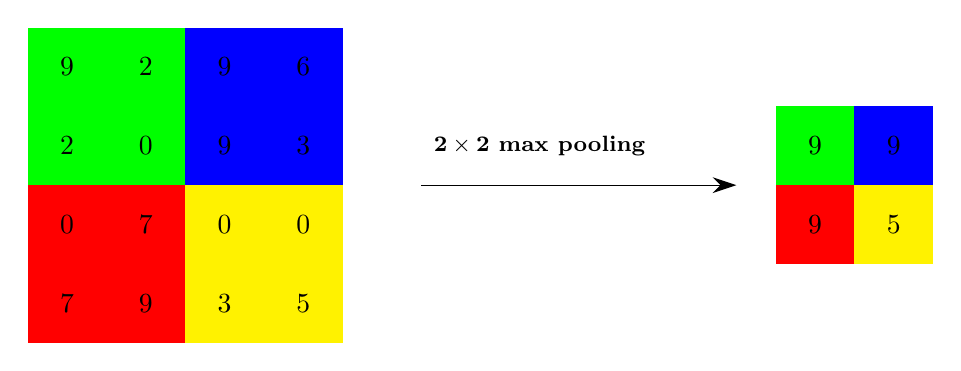
\begin{tikzpicture}
    \fill [red]    (0, 0)    rectangle (2, 2);
    \fill [yellow] (2, 0)    rectangle (4, 2);
    \fill [blue]   (2, 2)    rectangle (4, 4);
    \fill [green]  (0, 2)    rectangle (2, 4);

    \fill [red]    (9.5, 1)  rectangle (10.5, 2);
    \fill [yellow] (10.5, 1) rectangle (11.5, 2);
    \fill [blue]   (10.5, 2) rectangle (11.5, 3);
    \fill [green]  (9.5, 2)  rectangle (10.5, 3);

    \node at (0.5, 0.5) {7};
    \node at (1.5, 0.5) {9};
    \node at (2.5, 0.5) {3};
    \node at (3.5, 0.5) {5};
    %
    \node at (0.5, 1.5) {0};
    \node at (1.5, 1.5) {7};
    \node at (2.5, 1.5) {0};
    \node at (3.5, 1.5) {0};
    %
    \node at (0.5, 2.5) {2};
    \node at (1.5, 2.5) {0};
    \node at (2.5, 2.5) {9};
    \node at (3.5, 2.5) {3};
    %
    \node at (0.5, 3.5) {9};
    \node at (1.5, 3.5) {2};
    \node at (2.5, 3.5) {9};
    \node at (3.5, 3.5) {6};
    
    \node at (10, 1.5) {9};
    \node at (11, 1.5) {5};
    \node at (10, 2.5) {9};
    \node at (11, 2.5) {9};

    \draw[myarrow] (5, 2) -- (9,2);
    \node[font=\footnotesize\bfseries] at (6.5, 2.5) {$\mathbf{2\times 2}$ max pooling};
\end{tikzpicture}
 
    \captionof{figure}{Max Pooling}
    \label{fig:maxpooling}
\end{figure}

\subparagraph{Average Pooling}\mbox{}\\

Average Pooling consiste en tomar una ''ventana'' de la matriz de entrada y efectuar una operación fija que retorne un escalar. En este caso retorna el valor medio de la ventana y lo asigna como salida. A modo de ejemplo:\par

\begin{figure}[!h]
    \centering
    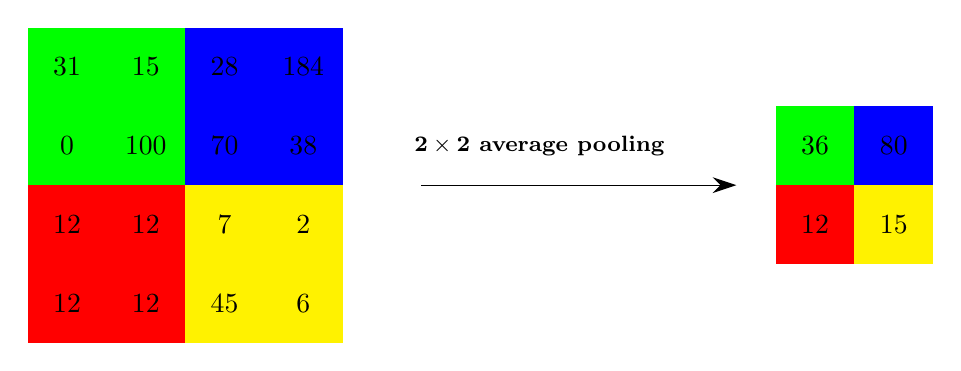
\begin{tikzpicture}
    \fill [red]    (0, 0)    rectangle (2, 2);
    \fill [yellow] (2, 0)    rectangle (4, 2);
    \fill [blue]   (2, 2)    rectangle (4, 4);
    \fill [green]  (0, 2)    rectangle (2, 4);

    \fill [red]    (9.5, 1)  rectangle (10.5, 2);
    \fill [yellow] (10.5, 1) rectangle (11.5, 2);
    \fill [blue]   (10.5, 2) rectangle (11.5, 3);
    \fill [green]  (9.5, 2)  rectangle (10.5, 3);

    \node at (0.5, 0.5) {12};
    \node at (1.5, 0.5) {12};
    \node at (2.5, 0.5) {45};
    \node at (3.5, 0.5) {6};
    %
    \node at (0.5, 1.5) {12};
    \node at (1.5, 1.5) {12};
    \node at (2.5, 1.5) {7};
    \node at (3.5, 1.5) {2};
    %
    \node at (0.5, 2.5) {0};
    \node at (1.5, 2.5) {100};
    \node at (2.5, 2.5) {70};
    \node at (3.5, 2.5) {38};
    %
    \node at (0.5, 3.5) {31};
    \node at (1.5, 3.5) {15};
    \node at (2.5, 3.5) {28};
    \node at (3.5, 3.5) {184};
    
    \node at (10, 1.5) {12};
    \node at (11, 1.5) {15};
    \node at (10, 2.5) {36};
    \node at (11, 2.5) {80};

    \draw[myarrow] (5, 2) -- (9,2);
    \node[font=\footnotesize\bfseries] at (6.5, 2.5) {$\mathbf{2\times 2}$ average pooling};
\end{tikzpicture}
 
    \captionof{figure}{Average Pooling}
    \label{fig:averagepooling}
\end{figure}

\paragraph{Capa de concatenación}\mbox{}\\

Esta capa es la encargada de tomar las entradas y concatenarlas a lo largo de una dimensión especifica, la única condición es que las entradas deben tener el mismo tamaño en todas las dimensiones excepto en la dimensión de concatenación.\par

\paragraph{Otras capas que suelen aparecer en una red neuronal convolucional}\mbox{}\\

Existen otras capas que suelen aparecer en algunas redes neuronales convolucionales como por ejemplo la capa de Dropout la cual consiste en desconectar un porcentaje de las neuronas en cada iteración del entrenamiento lo cual mejor la generalización de la red y ayuda a converger el entrenamiento.\par
La Normalización por lotes (mas conocida en ingles por ''Batch normalization'') que consiste en añadir un capa entre las neuronas y la función de activación para normalizar las activaciones de salida.\par
Existen algunas capas como la capa de convolución transpuesta (también conocida como capa de deconvolucion o capa de convolución fraccional) la cual se la utiliza para recuperar las dimensiones reducidas. Por ejemplo, luego de realizar una convolución con un step mayor que uno lo cual reduce el tamaño de la matriz de salida.\par


\subsubsection{Arquitectura de una red neuronal convolucional}

Una arquitectura de una red neuronal convolucional normalmente esta formada por una pila de capas distintas que transforman la matriz de entrada en una matriz de salida a través de una función diferenciable.\par
Algunas características importantes en las arquitecturas son: Los formatos de entrada/salida, la cantidad de capas de la red, parámetros de cada capa, la secuencia y forma de conexión de las capas entre si, y el algoritmo de entrenamiento. \par

Algunas redes y sus arquitecturas:

\begin{itemize}
    \item LeNet-5: 2 capas convolucionales y 3 ''fully connected''. Al rededor de 60.000 parámetros. Año 1998.
    \begin{center}
        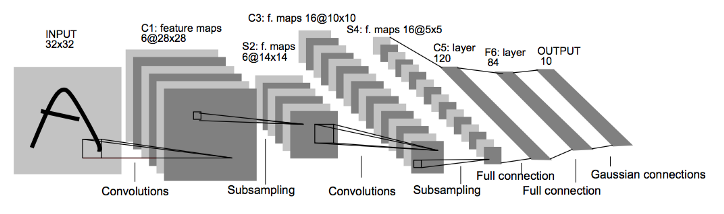
\includegraphics[scale=0.6]{Tesis/Capitulos/02_MARCO_TEORICO/img/LeNet5.png}
        \captionof{figure}{LeNet-5}
    \end{center}
    
    \item AlexNet: 8 capas, 3 ''fully connected'' y 5 convolucionales. Al rededor de 60 millones de parametros. Año 2012.
    
    \item VGG-16: 13 capas convolucionales y 3 ''fully connected''. Al rededor de 138 millones de parametros. Año 2014.
    
    \item ResNet-50: 50 capas, con modulos llamados ''ResNet'' (cada uno de 2 o 3 capas convolucionales). Al rededor de 26 millones de parametros. Año 2015.
    \begin{center}
        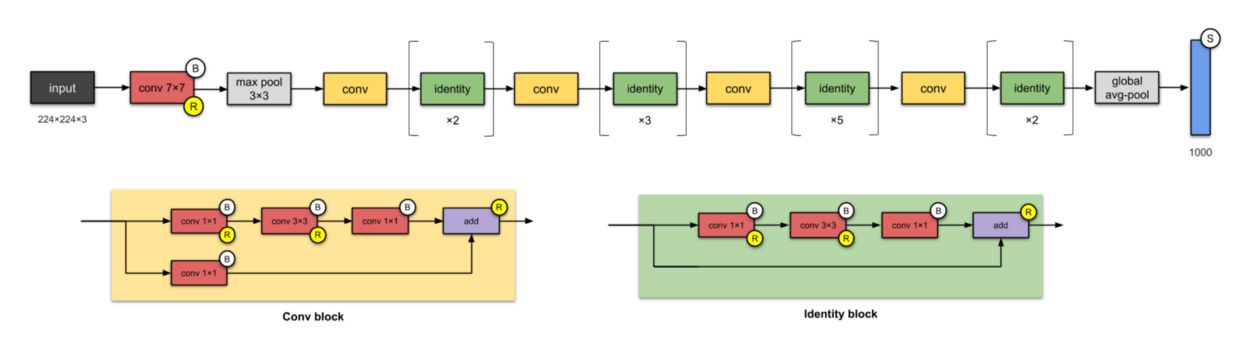
\includegraphics[scale=0.35]{Tesis/Capitulos/02_MARCO_TEORICO/img/ResNet50.png}
        \captionof{figure}{ResNet-50, de Raimi Karim, towardsdatascience}
    \end{center}
\end{itemize}

\subsubsection{Micro-arquitectura de una red neuronal convolucional}

La micro-arquitectura hace referencia a las capas individuales y/o módulos. A modo de ejemplo observemos el modulo ''ResNet'' de la red neuronal convolucionar ResNet-50.\par

\begin{figure}[H]
\hfill
\subfigure["Conv block" (Bloque de convolución)]{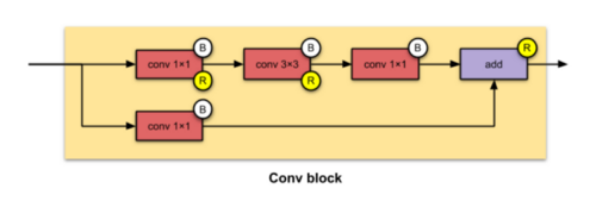
\includegraphics[width=5cm]{Tesis/Capitulos/02_MARCO_TEORICO/img/ResNetBlock1.png}}
\hfill
\subfigure[Identity block (Bloque de identidad)]{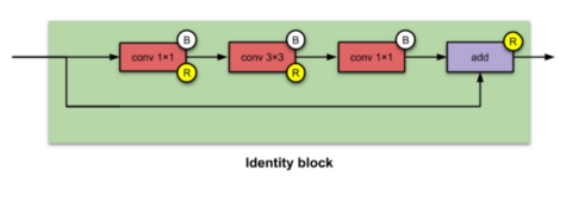
\includegraphics[width=5cm]{Tesis/Capitulos/02_MARCO_TEORICO/img/ResNetBlock2.png}}
\hfill
\caption{ResNet-50 modulo}
\end{figure}


\subsubsection{Entrenamiento de la red}

\paragraph{Introducción}\mbox{}\\

La fase de entrenamiento de la red neuronal convolucional consiste en, a partir de un set de imágenes de entrenamiento y sus respectivas etiquetas de los objetos a reconocer realizar iteraciones (también llamadas épocas) para ir determinando los pesos de cada uno de las neuronas en la red. Esta determinación se realiza a través del método de calculo conocido como ''Backpropagation''.\par
\bigbreak
Entonces en cada época, la etapa de entrenamiento se divide en dos etapas: Una fase directa (o hacia adelante) en donde una matriz de entrada pasa a través de toda la red neuronal. Se comparan las salidas obtenidas con las deseadas y se calcula el error para una de las salidas.\par
Y una fase inversa (o hacia atrás) donde los gradientes se pasan hacia atrás y los pesos se actualizan. Cada capa recibe un gradiente de perdida respecto a la salida y devuelve un gradiente de perdida respecto a la entrada. \par

Algo a tener en cuenta es que la fase de retroceso necesita datos que son almacenados durante la fase hacia adelante ya que se guardan datos de cada capas (entradas y valores intermedios) por lo que antes de realizar la propagación hacia atrás ''backpropagation'' es necesario una propagación hacia adelante ''forward propagation''. \par

\paragraph{Función de perdida}\mbox{}\\

Como mencione anteriormente finalizando la fase directa o de propagación hacia adelante se comparan las salidas obtenidas con las deseadas y se calcula el error para cada una de ellas. Esto se realiza a través de la Función de perdida $J_{(W)}$.\par
Es una tarea importante, en este proceso, la elección de la función de perdida que se va a minimizar. Ésta relaciona el valor esperado con los valores obtenido en la propagación hacia adelante.\par

\subparagraph{Entropía cruzada}\mbox{}\\

La entropía cruzada es una función de perdida típicamente utilizada para la clasificación de imágenes.\par

\begin{equation}
\tcboxmath[colback=white!25!white,colframe=black]
{ L = -ln(p_c) }  
\end{equation}

En donde ''c'' es la clase correcta y $p_c$ es la probabilidad predicha para la clase ''c''.\par

\paragraph{Desarrollo matemático}\mbox{}\\

Entonces, en la fase de la propagación hacia adelante, matemáticamente hablando se parte de una red en donde $a^{(l)}=f(z^{(l)})$ es la salida de la capa ''l'', tal que $z^{(l)}$ es el vector de pre-activación y se puede generalizar como $z^{(l)}=W^{(l)}*a^{(l-1)}$ siendo W los coeficientes de la capa y ''a'' la salida de la capa anterior y por ultimo $f()$, la función de activación de la capa l. \par
\bigbreak
Por otro lado, en la fase de propagación hacia atrás, matemáticamente hablando se utiliza un método de calculo de gradiente conocido como retropropagación y para poder utilizar este método es necesario encontrar las derivadas parciales de la función de perdida respecto a cada uno de los parámetros de la red $\frac{\partial J(W)}{\partial W^{l}_{ij}}$.\par

\begin{itemize}
    \item Se parte de Calcular el error y el delta de salida:
    \begin{enumerate}
        \item $e^{(L)} = d - a^{(L)}$ tal que ''L'' es la ultima capa, ''d'' el valor que debería dar a la salida y ''a'' el valor de la salida obtenido previamente en la propagación hacia adelante.
        \item $ \delta ^{(L)} = f'(z^{(L)}) \cdot e^{(L)}$ siendo $f'(z^{(L)}$ la derivada de la función de activación de la capa de salida.
    \end{enumerate}
    \item Para cada capa de la red neuronal se procede a calcular sus errores y deltas.
    \begin{enumerate}
        \item $e^{(L)} = W^{(l+1)^T} - \delta ^{(l+1)}$ tal que ''L'' es la ultima capa, ''d'' el valor que debería dar a la salida y ''a'' el valor de la salida obtenido previamente en la propagación hacia adelante.
        \item $ \delta ^{(L)} = f'(z^{(L)}) \cdot e^{(L)}$ siendo $f'(z^{(L)}$ la derivada de la función de activación de la capa de salida.
    \end{enumerate}
    \item Actualizamos las matrices de pesos.
    \begin{enumerate}
        \item $\Delta W^{(l)} = \lambda * (\delta^{(l)} \times a^{(l-1)} )$ tal que $\lambda$ se define como el factor de aprendizaje, y $a^{(l-1)}$ la salida de la neurona anterior.
        \item Actualización: $ W^{(l)} \leftarrow W^{(l)} + \Lambda W^{(l)} $
    \end{enumerate}
\end{itemize}

Este proceso se repite periódicamente (épocas) hasta alcanzar el entrenamiento deseado de la red.\par


% Lógica difusa
\newpage

\subsection{Lógica Difusa}

\subsubsection{Introducción}

A lo largo de los años hubo una gran cantidad de cambios en los paradigmas en las ciencias y matemáticas, en este caso me enfoco en el concepto de incertidumbre. Según la visión tradicional, la incertidumbre no era parte de la ciencia y esta se esforzaba en eliminarla. Según la visión alternativa, la incertidumbre juega un rol muy importante en la ciencia. \par
La lógica difusa fue investigada por primera vez por el ingeniero Lotfy A. Zadeh, en la Universidad de Berkeley (California) cuando logro comprender lo que el llamo principio de incompatibilidad: "A medida que aumenta la complejidad, las declaraciones precisas pierden significado y las declaraciones significativas pierden precisión". Lo que quiere decir es que cuando un sistema se vuelve mas complejo, nuestra capacidad de ser precisos disminuye (inherentemente debido a que la capacidad de la computación de datos no es infinita) mucho mas allá del cual la precisión y el significado son características indispensables.\par
La lógica difusa permite tomar decisiones mas o menos intensas en función de grados intermedios de cumplimiento de una premisa. Esta nueva lógica permite comprender nuestras expresiones del tipo <<hace mucho frió>>, <<él es un poco alto>>, <<su ritmo es algo lento>>, entre otras.\par
Este es uno de los temas que siempre aparece en cualquier documento, libro, artículos y/o revistas dedicada a los sistemas de control y se caracteriza por ser un sistema de control sencillo, robusto, económico, de muy rápida implementación y con la ventaja de que permite agregar múltiples entradas sin complejizar demasiado su resolución.\par

\subsubsection{Conjuntos difusos y funciones características}

Lotfy A. Zadeh utilizo el ejemplo de los hombres altos para poder explicar el concepto de conjunto difuso. Según la teoría clásica los hombres que superen cierta altura pertenecen al conjunto de hombres "altos". Así por ejemplo, tendríamos que cualquier hombre que supere 1,7 mts es considerado alto, en cambio quien pida 1,69 mts deja de considerado alto lo cual no tiene mucho sentido que un hombre sea considerado mientras que otro no cuando su altura difiere 1 cm. La lógica difusa propone un conjunto que no tiene una frontera clara, y asigna un cierto grado de pertenencia a ese conjunto, entre 0 y 1. Ejemplo: Un hombre que mida 1,49 mts tiene un grado de pertenencia del 0.8 al conjunto de hombres bajos, mientras que un hombre que mida 1.6 mts tiene un grado de pertenencia del 0.5 a este mismo conjunto.\par

\begin{center}
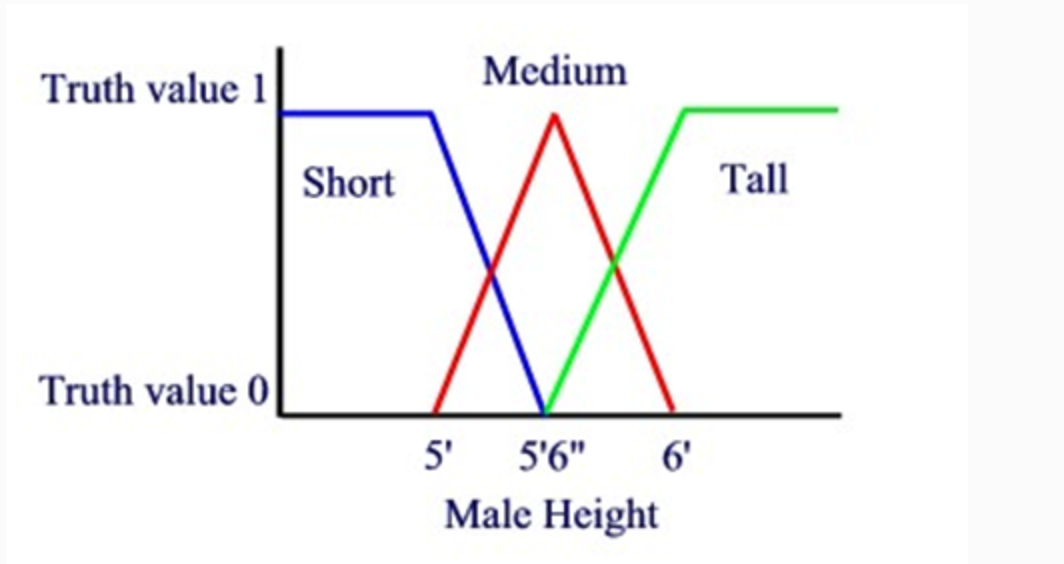
\includegraphics[scale=0.2]{Tesis/Capitulos/02_MARCO_TEORICO/img/ConjDifuso.png}
\captionof{figure}{Conjuntos difusos y funciones características}
\end{center}

Este grado de pertenencia de la persona en el conjunto se define mediante la función característica asociada al conjunto difuso. La función característica utilizada, depende del criterio que utilicemos para resolver nuestro problema. La única condición que debe cumplir una función característica es que tome valores entre 0 y 1 y sea continua.\par

Funciones características mas utilizadas: Gaussiana, Sigmoidal, Gamma, Pi, Campana, Trapezoidal, Triangular.\par

\begin{figure}[H]
    \centering
    \subfigure[]{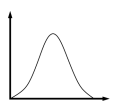
\includegraphics[width=0.2\textwidth]{Tesis/Capitulos/02_MARCO_TEORICO/img/gaussiana.png}} 
    \subfigure[]{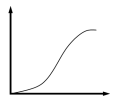
\includegraphics[width=0.2\textwidth]{Tesis/Capitulos/02_MARCO_TEORICO/img/logaritmica.png}} 
    \subfigure[]{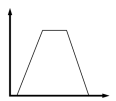
\includegraphics[width=0.2\textwidth]{Tesis/Capitulos/02_MARCO_TEORICO/img/trapezoidal.png}}
    \subfigure[]{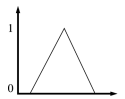
\includegraphics[width=0.2\textwidth]{Tesis/Capitulos/02_MARCO_TEORICO/img/triangular.png}}
    \caption{(a) Gaussiana (b) Sigmoidal (c) Trapezoidal (d) Triangular}
    \label{fig:foobar}
\end{figure}


\paragraph{Operaciones con conjuntos difusos}

\begin{itemize}
    \item Intersección:  \hfill 
    \begin{center}
        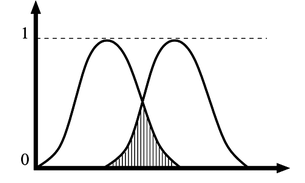
\includegraphics[scale=0.6]{Tesis/Capitulos/02_MARCO_TEORICO/img/interseccion.png}
        \captionof{figure}{Intersección }
    \end{center}
    \begin{equation}
    \tcboxmath[colback=white!25!white,colframe=black]
    {\mu( A \cap B ) (x) = min (\mu_A (x), \mu_B (x) )}  
    \end{equation}
    
    \item Unión:  \hfill 
    \begin{center}
        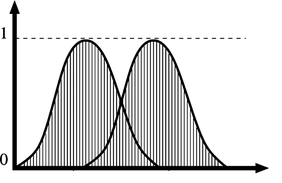
\includegraphics[scale=0.6]{Tesis/Capitulos/02_MARCO_TEORICO/img/union.png}
        \captionof{figure}{Unión }
    \end{center}
    \begin{equation}
    \tcboxmath[colback=white!25!white,colframe=black]
    {\mu( A \cup B ) (x) = max (\mu_A (x), \mu_B (x) )}  
    \end{equation}
    
    \item Complemento:  \hfill 
    \begin{center}
        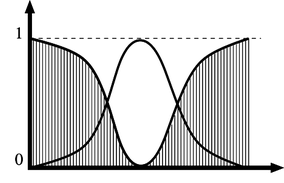
\includegraphics[scale=0.6]{Tesis/Capitulos/02_MARCO_TEORICO/img/complemento.png}
        \captionof{figure}{Complemento }
    \end{center}
    \begin{equation}
    \tcboxmath[colback=white!25!white,colframe=black]
    {\mu_A (x) = 1 - \mu_A (x)}  
    \end{equation}
    
    \item Inclusión:  \hfill  
    Un conjunto difuso, A, esta incluido en otro, B, si su función de pertenencia toma valores mas pequeños: 
    \begin{equation}
    \tcboxmath[colback=white!25!white,colframe=black]
    {\mu_B (x) \leq \mu_A (x)}  
    \end{equation}
    
\end{itemize}


\subsubsection{Reglas}

Se llama reglas difusas al conjunto de proposiciones IF-THEN que modelan el problema que uno planea resolver. Típicamente tienen la forma: \par
\bigbreak
    "Si v es A entonces c es B"
\bigbreak
Donde A y B son conjuntos difusos en los rangos de "v" y "c" respectivamente.
\bigbreak

El conjunto de reglas se definen en lenguaje natural, según el grado de pertenencia de sus variables será el grado de verdad de la regla. El comportamiento de la salida dependerá de las reglas con mayor grado de verdad.\par

\subsubsection{Control Difuso}

\begin{center}
    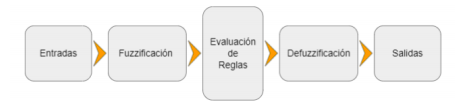
\includegraphics[scale=0.7]{Tesis/Capitulos/02_MARCO_TEORICO/img/etapas.png}
    \captionof{figure}{Proceso de control difuso}
\end{center}

Se puede descomponer el proceso de control difuso en tres etapas principales.\par

\paragraph{Fuzzificación} \label{fuzzymarker}

Primera parte del proceso, dados los valores de entrada se calcula el grado de pertenencia a cada uno de los conjuntos difusos considerados, mediante las funciones características asociadas a estos conjuntos difusos.\par

Por ejemplo, tomando la variable velocidad.\par

\begin{center}
    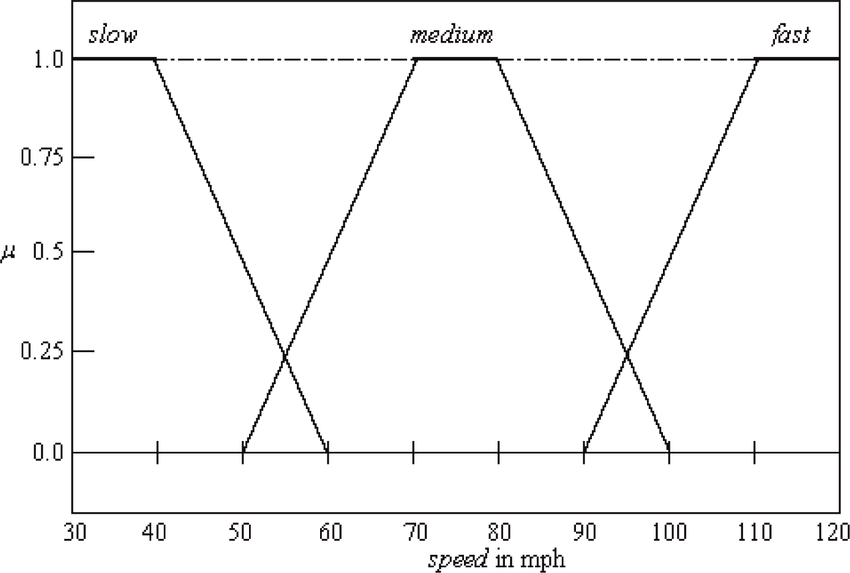
\includegraphics[scale=0.25]{Tesis/Capitulos/02_MARCO_TEORICO/img/speed.png}
    \captionof{figure}{Ejemplo Fuzzificación}
\end{center}

Con un valor de 65 mph, se cuantifica su grado de pertenencia a los conjuntos representados por algunas etiquetas lingüísticas: baja, media, alta. Para ellos se debió haber definido previamente una función de pertenencia para cada una de esas etiquetas que define que valores de la variable velocidad le pertenece y con que grado de pertenencia a cada una de ellas. Siguiendo con nuestro ejemplo, tiene un grado de pertenencia del 0 en la etiqueta ''baja''. Un grado de pertenencia del 0.75 en la etiqueta ''media'' y un 0 en la etiqueta ''alta''.\par

\paragraph{Evaluación de reglas}

Las reglas relacionan los conjuntos difusos de entrada mediante mecanismos de inferencia (reglas) con las salidas difusas.\par

Una vez terminada la etapa previa, la fuzzificación, se procede a evaluar los antecedentes de las reglas, obteniendo el grado de verdad o ''peso'' para cada una de ellas.\par

El peso de la regla estará dado por la veracidad del antecedente. Por ejemplo, si tiene una regla del tipo: \par

\begin{center}
\uline{\bfseries SI} la velocidad es ''baja'' \uline{\bfseries ENTONCES} ''aumente'' la potencia del motor.
\end{center}

Se asigna como peso el grado de pertenencia del valor leído de velocidad a la etiqueta lingüística "baja".

En el caso de que tenga una regla con conectivos lógicos \uline{\bfseries Y}:

\begin{center}
\uline{\bfseries SI} la velocidad es ''baja'' \uline{\bfseries Y} los obstáculos están ''lejos'' \uline{\bfseries ENTONCES} ''aumente'' la potencia del motor.
\end{center}

La regla sera tan verdadera como lo sea el menos verdadero de sus antecedentes. Por ende, se le asigna a la regla como peso, el menor de los grados de pertenencia de las variables de los antecedentes a las respectivas etiquetas lingüísticas.\par
Esto se repite para el resto de las reglas, entonces cada regla queda con su peso correspondiente.\par
\bigbreak
Así como cada entrada tiene sus propias funciones de pertenencia, cada salida le corresponde su propio set de funciones de pertenencia. Cada una de ella es una salida difusa (''baje'', ''no modifique'', ''aumente'' la potencia del motor).\par
\bigbreak
A cada una de las salidas difusas se les asigna un valor (grado de aplicabilidad) es el valor máximo de cada uno de los pesos de las reglas que la mencionan. De esta manera, tenemos casa salida difusa con su valor.

\paragraph{Defuzzificación}

De la etapa anterior del proceso tenemos varias salidas difusas (''baje'', ''aumente'') cada una de ellas con un valor de verdad o de aplicabilidad (un numero de 0 a 1) para cada conjunto difuso de cada salida del sistema (en este caso la potencia del motor).\par
\bigbreak
Ahora la pregunta es, cual es la potencia del motor? Una forma fácil y efectiva de determinarlo es realizando la operación denominada C.O.G (Centro de gravedad en ingles) el cual consiste en: \par

\begin{center}
\begin{equation}
        \tcboxmath[colback=white!25!white,colframe=black]
        { u = \frac{ \int_{}^{} u. \mu(u) \cdot du }{ \int_{}^{} \mu(u) \cdot du } }  
\end{equation}
\end{center}

Ejemplo del método "Centro de gravedad" \par

\begin{center}
    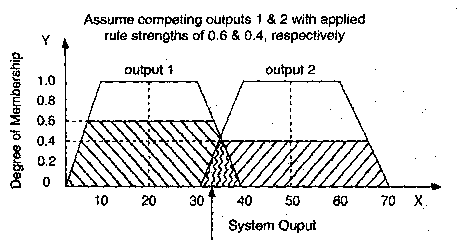
\includegraphics[scale=0.7]{Tesis/Capitulos/02_MARCO_TEORICO/img/COG.png}
    \captionof{figure}{Ejemplo C.O.G}
\end{center}

\underline{\textbf{Método del Centro de gravedad (C.O.G)}} (asumiendo que los pesos de las reglas 1 y 2 son 0.6 y 0.4 respectivamente)

\begin{itemize}
    \item Se determina el centroide de la función de pertenencia de salida. En este caso seria X=20 para la salida 1 y X=50 para la salida 2.
    \item Las funciones de pertenencia están limitadas en altura por el peso de la regla aplicada, y se calculan las áreas de las funciones de pertenencias (Área del trapecio $A=\frac{B+b}{2}.h$ ).\par
    Área de la salida 1: $A_1 =\frac{40+28}{2}.0.6 = 20.4 $ \par
    Área de la salida 2: $A_2 =\frac{40+32}{2}.0.4 = 14.4 $ \par
    \item Finalmente la salida defuzzificada es el promedio ponderado de los centroides y las áreas calculadas: Peso promedio: $W_{av} =\frac{20*20.4+14.4*50}{20.4+14.4} = 32.4 $
\end{itemize}

\underline{\textbf{Utilizando Singletons}} (asumiendo que los pesos de las reglas 1 y 2 son 0.6 y 0.4 respectivamente)

Con el propósito de simplificar el proceso de defuzzificación se utiliza un Singleton (una función de pertenencia de salida representada por una única linea vertical). De esta forma el calculo del centro de gravedad se traduce en un único calculo promedio ponderado entre los centroides y la aplicabilidad de las reglas: $W_{av} =\frac{20*0.6+50*0.4}{0.6+0.4} = 32.0 $

% Sistema Integrado
\newpage
\subsection{Sistema Integrado}

%\subsubsection{Introducción}

    % Chapter 1
    \newpage
    \hypersetup{hidelinks}
    \section{MODULO: SISTEMA DE CONTROL DIFUSO}

\subsection{Simulación de la planificación de movimiento}

Como se mencionó anteriormente el problema se puede clasificar dentro de los de planificación de movimiento (motion planning), se debe mover un objeto (robot) desde un punto inicial a un punto final evitando colisionar con los posibles obstáculos del entorno. El robot conoce su pose (el ángulo hacia dónde se orienta respecto al eje de coordenadas) en todo momento y el ángulo hacia el target, además no presenta limitaciones en cuanto al ángulo de giro. La detección de obstáculos se realiza mediante tres sensores de distancia.

Algunas consideraciones que se tuvieron en cuenta para el armado de reglas y funciones de pertenencia [6].

\begin{itemize}
    \item Cubrir adecuadamente el espacio de estado del problema.
    \item El conjunto de reglas debe ser completo y correcto.
    \item Las reglas no deben ser contradictorias.
    \item Para todos los valores de entrada la suma del grado de pertenencia de los distintos conjuntos debe ser 1.
\end{itemize}

\subsubsection{Módulos de control propuestos}

El desarrollo de la solución se puede dividir en versiones que van desde menor a mayor complejidad. Partiendo de un ejemplo de simulación y control difuso implementado en matlab que muestra como ajustar un sistema de lógica difusa usando una función de costo personalizada y que se puede encontrar \href{https://www.mathworks.com/help/fuzzy/tune-fuzzy-systems-using-custom-cost-function.html}{\textbf{aqui}}, a partir de ahora llamado "MySimAvoidObs1".

\paragraph{MySimAvoidObs1}\mbox{}\\

Nuestra idea base, fue controlar con el sistema difuso la variación del ángulo actual del robot para evadir un obstáculo. En este planteo el robot no tiene información sobre el destino, solo se encarga de evadir obstáculos. De este modo se representa el control con el siguiente esquema.

\subparagraph{Variables MySimAvoidObs1}\mbox{}\\


\paragraph{MySimAvoidObs2}\mbox{}\\

\begin{center}
    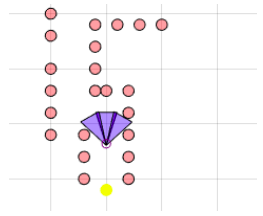
\includegraphics[scale=0.5]{Tesis/Capitulos/04_CAPITULO_2/img/des1.png}
    \captionof{figure}{Captura de la simulacion de MySimAvoidObs2.}
\end{center}

\begin{center}
    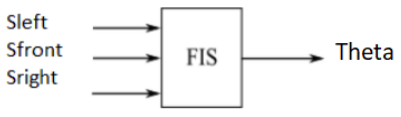
\includegraphics[scale=0.5]{Tesis/Capitulos/04_CAPITULO_2/img/esquema1.png}
    \captionof{figure}{Esquema de entradas y salidas MySimAvoidObs2.}
\end{center}

En donde Sleft, Sfront, y Sright representa las distancias al obstáculo y Theta el ángulo que deberá girar el robot para evadirlo.

\subparagraph{Variables MySimAvoidObs2}\mbox{}\\

A continuación se muestra el detalle de las funciones de pertenencia de las variables intervinientes en el control difuso. Consideramos como entradas la distancia al obstáculo obtenida mediante tres sensores con ángulo ajustable. En los tres sensores se repiten las funciones “cerca” y “lejos”.

    % Chapter 2
    \newpage
    \hypersetup{hidelinks}
    \section{MODULO: PROCESAMIENTO DE IMÁGENES}
    
    % Chapter 3
    \newpage
    \hypersetup{hidelinks}
    \section{SISTEMA INTEGRADO}
    
    % Resultados
    \newpage
    \hypersetup{hidelinks}
    \section{RESULTADOS}



    
    % Conclusión
    \newpage
    \hypersetup{hidelinks}
    \section{CONCLUSIÓN}

asdasd

    % 00. Matriz de requisitos
    \newpage
    \hypersetup{hidelinks}
    \begin{landscape}
\section{APÉNDICE A}
\subsection{Matriz de requisitos}

\begin{tabular}{| l | m{4.5cm} | c | c | c | c | c | m{5.5cm} |}
    \hline
    \multicolumn{8}{ |c| }{Matriz de requisitos} \\ 
    \hline
    \multicolumn{1}{|c|}{ID}  & \multicolumn{1}{c|}{Requisito} & \multicolumn{3}{c|}{Estado completo}  & \multicolumn{1}{c|}{Prioridad} & \multicolumn{1}{c|}{Complejidad} & \multicolumn{1}{c|}{Objetivo} \\ 

    \cline{1-8}    
    & & Estado & Versión & Fecha & & & \\  
    %%%%%%%%%%%%%%%%%%%%%%%%%%%%%%%%%%%%%%%%%%%%%%%%%%%%%%%%%%%%%%%%%%%%%%%%%%%%%%%
    %%%%%%%%%%%%%%%%%%%%%%%%%%%%%%%%%%%%%%%%%%%%%%%%%%%%%%%%%%%%%%%%%%%%%%%%%%%%%%%
    0 &                                                 % ID
    Tiene que reconocer obstáculos. &           % Requisito
    \cellcolor{yellow}  EN CURSO  & 1.0 & \today &      % Estado
    ALTA &                                              % Prioridad
    ALTA &                                              % Complejidad
                                                        % Objetivo
    Capacidad de reconocer algunos de los obstáculos.\\\hline
    %%%%%%%%%%%%%%%%%%%%%%%%%%%%%%%%%%%%%%%%%%%%%%%%%%%%%%%%%%%%%%%%%%%%%%%%%%%%%%%
    %%%%%%%%%%%%%%%%%%%%%%%%%%%%%%%%%%%%%%%%%%%%%%%%%%%%%%%%%%%%%%%%%%%%%%%%%%%%%%%
    1 &                                                 % ID
    Tiene que evadir obstáculos. &                      % Requisito
    \cellcolor{yellow} EN CURSO & 1.0 & \today &        % Estado
    ALTA &                                              % Prioridad
    ALTA &                                              % Complejidad
                                                        % Objetivo
    Capacidad de evadir obstáculos, si el obstáculo es reconocido la evasión se hará en función de sus dimensiones.\\\hline
    %%%%%%%%%%%%%%%%%%%%%%%%%%%%%%%%%%%%%%%%%%%%%%%%%%%%%%%%%%%%%%%%%%%%%%%%%%%%%%%
    %%%%%%%%%%%%%%%%%%%%%%%%%%%%%%%%%%%%%%%%%%%%%%%%%%%%%%%%%%%%%%%%%%%%%%%%%%%%%%%
    2 &                                                 % ID
    Capacidad de desplazarse.   &                       % Requisito
    \cellcolor{red} SIN COMENZAR & 1.0 & \today &       % Estado
    ALTA &                                              % Prioridad
    BAJA &                                              % Complejidad
                                                        % Objetivo
    Capacidad de desplazarse a través de ciertos entornos.\\\hline   
    %%%%%%%%%%%%%%%%%%%%%%%%%%%%%%%%%%%%%%%%%%%%%%%%%%%%%%%%%%%%%%%%%%%%%%%%%%%%%%%
    %%%%%%%%%%%%%%%%%%%%%%%%%%%%%%%%%%%%%%%%%%%%%%%%%%%%%%%%%%%%%%%%%%%%%%%%%%%%%%%
    3 &                                                 % ID
    Capacidad de sensar distancia a obstáculos.   &     % Requisito
    \cellcolor{red} SIN COMENZAR & 1.0 & \today &       % Estado
    ALTA &                                              % Prioridad
    BAJA &                                              % Complejidad
                                                        % Objetivo
    Necesidad de obtener la distancia al obstáculo en su cono de visión.\\\hline   
    %%%%%%%%%%%%%%%%%%%%%%%%%%%%%%%%%%%%%%%%%%%%%%%%%%%%%%%%%%%%%%%%%%%%%%%%%%%%%%%
    %%%%%%%%%%%%%%%%%%%%%%%%%%%%%%%%%%%%%%%%%%%%%%%%%%%%%%%%%%%%%%%%%%%%%%%%%%%%%%%
    4 &                                                 % ID
    Capacidad de conocer dirección de desplazamiento. & % Requisito
    \cellcolor{red} SIN COMENZAR & 1.0 & \today &       % Estado
    ALTA &                                              % Prioridad
    MEDIA &                                             % Complejidad
                                                        % Objetivo
    Necesidad de saber el sentido al cual se dirige.\\\hline
    %%%%%%%%%%%%%%%%%%%%%%%%%%%%%%%%%%%%%%%%%%%%%%%%%%%%%%%%%%%%%%%%%%%%%%%%%%%%%%%
    %%%%%%%%%%%%%%%%%%%%%%%%%%%%%%%%%%%%%%%%%%%%%%%%%%%%%%%%%%%%%%%%%%%%%%%%%%%%%%%
    5 &                                                 % ID
    Capacidad de medir la distancia recorrida.  &       % Requisito
    \cellcolor{red} SIN COMENZAR & 1.0 & \today &       % Estado
    ALTA &                                              % Prioridad
    MEDIA &                                             % Complejidad
                                                        % Objetivo
    Decoders ayudarán a medir la distancia recorrida.\\\hline
    %%%%%%%%%%%%%%%%%%%%%%%%%%%%%%%%%%%%%%%%%%%%%%%%%%%%%%%%%%%%%%%%%%%%%%%%%%%%%%%
    %%%%%%%%%%%%%%%%%%%%%%%%%%%%%%%%%%%%%%%%%%%%%%%%%%%%%%%%%%%%%%%%%%%%%%%%%%%%%%%
    6 &                                                 % ID
    Tiene que ser implementado en la Zybo.  &       % Requisito
    \cellcolor{red} SIN COMENZAR & 1.0 & \today &       % Estado
    BAJA &                                              % Prioridad
    MEDIA &                                             % Complejidad
                                                        % Objetivo
    Implementado en la placa de desarrollo Zybo.\\\hline
    %%%%%%%%%%%%%%%%%%%%%%%%%%%%%%%%%%%%%%%%%%%%%%%%%%%%%%%%%%%%%%%%%%%%%%%%%%%%%%%
    %%%%%%%%%%%%%%%%%%%%%%%%%%%%%%%%%%%%%%%%%%%%%%%%%%%%%%%%%%%%%%%%%%%%%%%%%%%%%%%
    7 &                                                 % ID
    Tiene que ser alimentado por batería.  &       % Requisito
    \cellcolor{red} SIN COMENZAR & 1.0 & \today &       % Estado
    BAJA &                                              % Prioridad
    BAJA &                                             % Complejidad
                                                        % Objetivo
    -.\\\hline
    %%%%%%%%%%%%%%%%%%%%%%%%%%%%%%%%%%%%%%%%%%%%%%%%%%%%%%%%%%%%%%%%%%%%%%%%%%%%%%%
    %%%%%%%%%%%%%%%%%%%%%%%%%%%%%%%%%%%%%%%%%%%%%%%%%%%%%%%%%%%%%%%%%%%%%%%%%%%%%%%
    8 &                                                 % ID
    Operaciones de mayor consumo computacional tienen que ser implementadas en una FPGA.  &                                            % Requisito
    \cellcolor{yellow} EN CURSO & 1.0 & \today &       % Estado
    BAJA &                                              % Prioridad
    ALTA &                                              % Complejidad
                                                        % Objetivo
    Con el propósito de ahorrar energía, acelerar las operaciones, etc.\\\hline
    %%%%%%%%%%%%%%%%%%%%%%%%%%%%%%%%%%%%%%%%%%%%%%%%%%%%%%%%%%%%%%%%%%%%%%%%%%%%%%%
    %%%%%%%%%%%%%%%%%%%%%%%%%%%%%%%%%%%%%%%%%%%%%%%%%%%%%%%%%%%%%%%%%%%%%%%%%%%%%%%
    
\end{tabular}
\end{landscape}


    % 01. Gantt
    \newpage
    \hypersetup{hidelinks}
    \begin{landscape}
    \subsection{Diagrama de Gantt}
    \begin{figure}[ht]
    	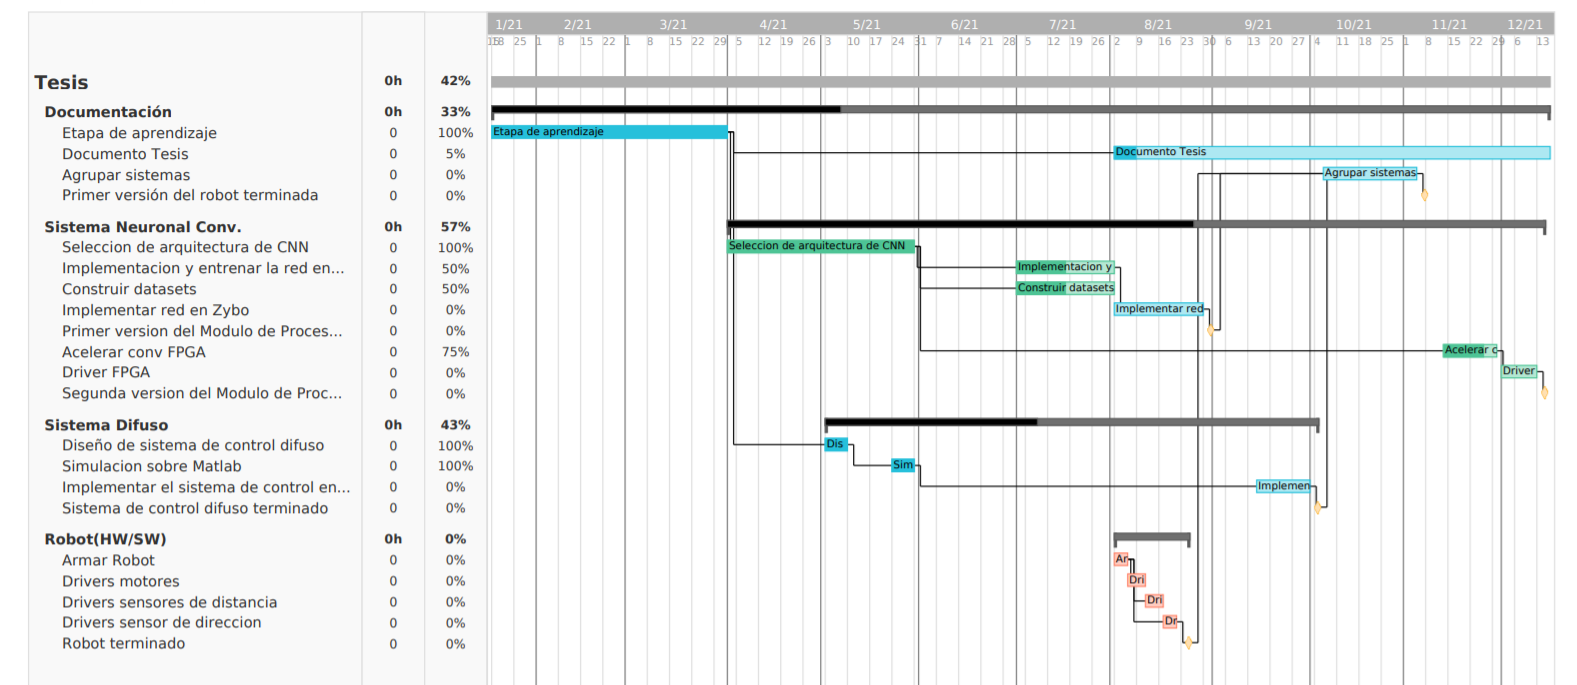
\includegraphics[width=0.95\linewidth]{Tesis/Capitulos/APENDICE_A/img/Gantt.png}
    	\caption{Diagrama de Gantt}
    	\label{fig:diagrama}
	\end{figure} 
\end{landscape}


    % 02. Riesgos
    \newpage
    \hypersetup{hidelinks}
    \subsection{Gestión del riesgo}

La matriz de probabilidad-impacto es una herramienta de análisis cualitativo de riesgos que nos permite establecer prioridades en cuanto a los posibles riesgos de un proyecto en función tanto de la probabilidad de que ocurran como de las repercusiones que podrían tener sobre nuestro proyecto en caso de que ocurrieran.\\

\centering {RIESGO = Probabilidad x Impacto}

\begin{table}[h!]
    \begin{center}
    \begin{tabular}{| c | c | c | c | c | c | c | c | }
        \hline
        \multicolumn{3}{ |c  }{}                            & \multicolumn{5}{ |c| }{Probabilidad}                                                      \\ \hline
        \multicolumn{3}{ |c| }{}                            & Excepcional          & Poco probable        & Probable             & Muy probable         & Inminente     \\ \hline
        \multicolumn{3}{ |c| }{}                            & (2)                  & (4)                  & (6)                  & (8)                  & (10)          \\ \hline
        \multirow{5}{*}{Impacto} & Extensiva     & (10)     & 20\cellcolor{yellow} & 40\cellcolor{yellow} & 60\cellcolor{red} & 80\cellcolor{red}    & 100\cellcolor{red} \\
                                 & Mayor         & (8)      & 16\cellcolor{green} & 32\cellcolor{yellow} & 48\cellcolor{yellow} & 64\cellcolor{red}    & 80 \cellcolor{red} \\
                                 & Localizada    & (6)      & 12\cellcolor{green}  & 24\cellcolor{yellow} & 36\cellcolor{yellow} & 48\cellcolor{yellow} & 60 \cellcolor{red} \\
                                 & Menor         & (4)      & 08\cellcolor{green}  & 16\cellcolor{green}  & 24\cellcolor{yellow} & 32\cellcolor{yellow} & 40 \cellcolor{red} \\
                                 & Leve          & (2)      & 04\cellcolor{green}  & 08\cellcolor{green}  & 12\cellcolor{green} & 16\cellcolor{yellow} & 20 \cellcolor{yellow} \\\hline
    \end{tabular}
        \caption{\centering Matriz de probabilidad por impacto}
        \label{tab:coches}
    \end{center}
\end{table}


\begin{table}[h!]
    \centering
    \begin{tabular}{|p{2cm}|p{10cm}|}
        \hline \bf Colour & \bf Legenda \\
        \hline \cellcolor{red} & No aceptable, se requiere reducción del riesgo. \\ [10pt]
        \hline \cellcolor{yellow} & Aceptable pero considere reducción del riesgo. \\[10pt]
        \hline \cellcolor{green} & Aceptable. \\ [10pt]
        \hline
    \end{tabular}
    \caption{Leyenda de colores de la matriz de riesgo}
\end{table}


\flushleft \subsubsection{Riesgos técnicos}

    \begin{itemize}
        \item[•] Incorrecta selección de arquitectura de la red neuronal convolucional y/o modificación de las etapas necesarias (24)
        \begin{itemize}
            \item[·] Si bien es muy probable que la red a utilizar sea seleccionada en función a la cantidad de recursos disponible para poder implementarla, este riesgo puede ocasionar una reimplementación a nivel de software o hardware. Por lo tanto este riesgo tiene una probabilidad de ocurrencia \textbf{PROBABLE} y un impacto \textbf{MENOR}.\\
            \textbf{Gestión:} Mitigación, se reducirán las probabilidad de ocurrencia al mínimo con mucha investigación previa. 
        \end{itemize}
        
        \item[•] Aprendizaje mayor al esperado (80)
        \begin{itemize}
            \item[·] Gran parte del desarrollo se llevara acabo sobre la placa de desarrollo ZYBO (Zynq Board). Durante la carrera el complejo tipo de SOC jamás fue utilizado. 
            Además el conocimiento requerido en temas como Fuzzy Logic, redes neuronales, redes neuronales convolucionales, y HDL fueron temas solo alcanzados en algunas materias de forma muy limitada y/o jamas vistos. Este riesgo tiene una probabilidad de ocurrencia \textbf{INMINENTE} y un impacto \textbf{MAYOR}.\\
            \textbf{Gestión:} Mitigación, se reducirán las probabilidad de ocurrencia al mínimo con mucha investigación previa. 
        \end{itemize}
        
        \item[•] Sensibilidad, precisión, y calidad de los sensores (32)
        \begin{itemize}
            \item[·] Este riesgo puede ocasionar que los resultados esperados del sistema de control difuso no sea el esperado. Este riesgo tiene una probabilidad de ocurrencia \textbf{MUY PROBABLE} y un impacto \textbf{MENOR}.\\
            \textbf{Gestión:} El propio sistema de control difuso mitiga la precisión de los sensores por ser un sistema de control robusto.
        \end{itemize}
        
        \item[•] Capacidad de reconocer la dirección de avance del robot (60)
        \begin{itemize}
            \item[·] Este riesgo es uno de los mas grandes a enfrentar, ya que el gps no brinda buenos resultados en interiores, además es necesario conocer la orientación del robot y la ubicación del target o objetivo a alcanzar.
            Este riesgo también puede ocasionar que los resultados esperados del sistema de control difuso no sea el esperado. Este riesgo tiene una probabilidad de ocurrencia \textbf{INMINENTE} y un impacto \textbf{LOCALIZADO}.\\
            \textbf{Gestión:} Se intentará buscar una forma óptima de geolocalización o bien simplemente el usuario definirá un punto relativo a la orientación y ubicación inicial del robot, utilizando unos decoders en los motores del robot y una brújula para conocer la dirección de avance. 
        \end{itemize}
        
        \item[•] Imposibilidad de implementar el acelerado del sistema de reconocimiento del robot por hardware (16)
        \begin{itemize}
            \item[·] Previendo problemas al realizar la implementación y por falta de tiempo. Este riesgo tiene una probabilidad de ocurrencia \textbf{MUY PROBABLE} y un impacto \textbf{LEVE}.\\
            \textbf{Gestión:} Aceptación, se aceptaran las consecuencias del riesgo. 
        \end{itemize}
        
        \item[•] Reducción de la exactitud de la red neuronal convolucional al utilizar aritmética de punto fijo (12)
        \begin{itemize}
            \item[·] Normalmente los parámetros de una red neuronal convolucional son flotantes de 32 o 64 bits. En caso de implementar algunas operaciones sobre la FPGA sera necesario reducir la representación a 8 bits con punto fijo, lo que provocara una reducción de la calidad de la precisión de la red. Se puede mitigar con correctas simulaciones sobre la PC y reentrenando la red. Este riesgo tiene una probabilidad de ocurrencia \textbf{PROBABLE} y un impacto \textbf{LEVE}.\\
            \textbf{Gestión:} Mitigación, existen distintos programas para prever la precisión que tendrá la red al ser implementada con aritmética de 8 bits de punto fijo.
        \end{itemize}
        
         \item[•] Dificultad al integrar los módulos desarrollados por separado y de alcanzar el objetivo esperado (80)
        \begin{itemize}
            \item[·] Una vez finalizado el sistema de control difuso y el modulo de procesamiento de imágenes existe el riesgo de redefinir algunas partes de los módulos para poder integrarlos. A su vez existe la posibilidad, una vez integrados los sistemas de no lograr el resultado esperado del proyecto. Este riesgo tiene una probabilidad de ocurrencia \textbf{MUY PROBABLE} y un impacto \textbf{EXTENSIVO}.\\
            \textbf{Gestión:} En caso de que mi sistema de navegación no obtenga los resultados esperado y el sistema de procesamiento de imágenes no complemente y/o realce los beneficios del sistema difuso (extienda sus capacidades) no se va a asumir ninguna acción ya que es un resultado completamente válido para un proyecto de investigación. Y simplemente se remarcara en la tesis que por ahí no es el camino.
        \end{itemize}
        
    \end{itemize}


\subsubsection{Riesgos organizativos}

    \begin{itemize}
        \item[•] Disponibilidad del hardware (16)
        \begin{itemize}
            \item[·] Al ser un hardware caro afrontado por mi, y quiza eventualmente provisto por la facultad. Este riesgo tiene una probabilidad de ocurrencia \textbf{EXCEPCIONAL} y un impacto \textbf{MAYOR}.\\
            \textbf{Gestión:} Prevención, esta amenaza se eliminara adquiriendo la placa de desarrollo.
        \end{itemize}
        
        \item[•] Errores de estimación del cronograma (48)
        \begin{itemize}
            \item[·] Este riesgo puede aparecer por desconocimiento y falta de experiencia en este tipo de desarrollos. Este riesgo puede ocasionar que no se llegue a cumplir con las fechas de los hitos del proyecto. Este riesgo tiene una probabilidad de ocurrencia \textbf{PROBABLE} y un impacto \textbf{MAYOR}.
        \end{itemize}
    
        \item[•] Priorizar inadecuadamente las tareas del proyecto (48)
        \begin{itemize}
            \item[·] Este riesgo puede aparecer si se elige incorrectamente el orden de prioridad de las tareas del proyecto, ocasionando que ciertas tareas que deberían ser necesarias para el desarrollo de otras no estén terminadas. Este riesgo tiene una probabilidad de ocurrencia \textbf{PROBABLE} y un impacto \textbf{MAYOR}.
        \end{itemize}
        
        \item[•] Omisión de tareas en el cronograma (48)
        \begin{itemize}
            \item[·] Pueden existir tareas que debido a su poca carga de trabajo, no hayan sido tomadas en cuenta dentro del cronograma. Esto puede ocasionar retrasos no contemplados dentro del proyecto. Este riesgo tiene una probabilidad de ocurrencia \textbf{PROBABLE} y un impacto \textbf{MAYOR}.
        \end{itemize}
    \end{itemize}

\subsubsection{Riesgos externos}  
    
    \begin{itemize}
        \item[•] Cuarentena (80)
        \begin{itemize}
            \item[·] Ante la actual situación epidemiológica nacional e internacional en relación con la infección por coronavirus (Covid-19) se pueden encontrar problemas a la hora de acceder a recursos necesarios que podría proveer la facultad. Este riesgo tiene una probabilidad de ocurrencia \textbf{INMINENTE} y un impacto \textbf{MAYOR}.
        \end{itemize}
    \end{itemize}
    
    \newpage

    \begin{table}[h!]
        \scriptsize
        \hspace{-1.5cm}
        \begin{tabular}{ p{3cm} c c c c p{4cm} p{4cm} }
            \\\hline 
            \bf \bf Riesgo & \bf ID & \bf Probabilidad & \bf Impacto & \bf Riesgo & \bf Detalle & \bf Gestión \\
            \hline
            
            &&&&&&\\
            Incorrecta selección de arquitectura de la red neuronal convolucional y/o modificación de las etapas necesarias &
            0 &
            PROBABLE &
            MENOR &
            24\cellcolor{yellow} &
            Si bien es muy probable que la red a utilizar sea seleccionada en función a la cantidad de recursos disponible para poder implementarla, este riesgo puede ocasionar una reimplementación a nivel de software o hardware.  & 
            Mitigación, se reducirán las probabilidad de ocurrencia al mínimo con mucha investigación previa. 
            \\\\\hline 
            
            &&&&&&\\
            Aprendizaje mayor al esperado &
            1 &
            INMINENTE &
            MAYOR &
            80\cellcolor{red} &
            Gran parte del desarrollo se llevara acabo sobre la placa de desarrollo ZYBO (Zynq Board). Durante la carrera el complejo tipo de SOC jamás fue utilizado. 
            Además el conocimiento requerido en temas como Fuzzy Logic, redes neuronales, redes neuronales convolucionales, y HDL fueron temas solo alcanzados en algunas materias de forma muy limitada y/o jamas vistos.  & 
            Mitigación, se reducirán las probabilidad de ocurrencia al mínimo con mucha investigación previa. 
            \\\\\hline 

            &&&&&&\\
            Sensibilidad, precisión, y calidad de los sensores &
            2 &
            MUY PROBABLE &
            MENOR &
            32\cellcolor{yellow} &
            Este riesgo puede ocasionar que los resultados esperados del sistema de control difuso no sea el esperado.  & 
            El propio sistema de control difuso mitiga la precisión de los sensores por ser un sistema de control robusto.  
            \\\\\hline 
            
            &&&&&&\\
            Capacidad de reconocer la dirección de avance del robot &
            3 &
            INMINENTE &
            LOCALIZADO &
            60\cellcolor{red} &
            Este riesgo es uno de los mas grandes a enfrentar, ya que el gps no brinda buenos resultados en interiores, además es necesario conocer la orientación del robot y la ubicación del target o objetivo a alcanzar.
            Este riesgo también puede ocasionar que los resultados esperados del sistema de control difuso no sea el esperado. & 
            Se intentará buscar una forma óptima de geolocalización o bien simplemente el usuario definirá un punto relativo a la orientación y ubicación inicial del robot, utilizando unos decoders en los motores del robot y una brújula para conocer la dirección de avance.   
            \\\\\hline  
            
            &&&&&&\\
            Imposibilidad de implementar el acelerado del sistema de reconocimiento del robot por hardware &
            4 &
            PROBABLE &
            LEVE &
            12\cellcolor{green} &
            Previendo problemas al realizar la implementación y por falta de tiempo. & 
            Aceptación, se aceptaran las consecuencias del riesgo.  
            \\\\\hline  
            
            &&&&&&\\
            Reducción de la exactitud de la red neuronal convolucional al utilizar aritmética de punto fijo &
            5 &
            PROBABLE &
            LEVE &
            12\cellcolor{green} &
            Normalmente los parámetros de una red neuronal convolucional son flotantes de 32 o 64 bits. En caso de implementar algunas operaciones sobre la FPGA sera necesario reducir la representación a 8 bits con punto fijo, lo que provocara una reducción de la calidad de la precisión de la red. Se puede mitigar con correctas simulaciones sobre la PC y reentrenando la red. & 
            Mitigación, existen distintos programas para prever la precisión que tendrá la red al ser implementada con aritmética de 8 bits de punto fijo.  
            \\\\ 

        \end{tabular}
    \end{table}

\newpage

\begin{table}[h!]
        \scriptsize
        \hspace{-1.5cm}
        \begin{tabular}{ p{3cm} c c c c p{4cm} p{4cm} }
            \\\hline 
            \bf \bf Riesgo & \bf ID & \bf Probabilidad & \bf Impacto & \bf Riesgo & \bf Detalle & \bf Gestión \\
            \hline
            
            &&&&&&\\
            Dificultad al integrar los módulos desarrollados por separado y de alcanzar el objetivo esperado &
            6 &
            MUY PROBABLE &
            EXTENSIVO &
            80\cellcolor{red} &
            Una vez finalizado el sistema de control difuso y el modulo de procesamiento de imágenes existe el riesgo de redefinir algunas partes de los módulos para poder integrarlos. A su vez existe la posibilidad, una vez integrados los sistemas de no lograr el resultado esperado del proyecto. & 
            En caso de que mi sistema de navegación no obtenga los resultados esperado y el sistema de procesamiento de imágenes no complemente y/o realce los beneficios del sistema difuso (extienda sus capacidades) no se va a asumir ninguna acción ya que es un resultado completamente válido para un proyecto de investigación. Y simplemente se remarcara en la tesis que por ahí no es el camino.
            \\\\\hline 
            
            &&&&&&\\
            Disponibilidad del hardware &
            7 &
            EXCEPCIONAL &
            MAYOR &
            16\cellcolor{green} &
            Al ser un hardware caro afrontado por mi, y quiza eventualmente provisto por la facultad. & 
            Prevención, esta amenaza se eliminara adquiriendo la placa de desarrollo.
            \\\\\hline 
            
            &&&&&&\\
            Errores de estimación del cronograma &
            8 &
            PROBABLE &
            MAYOR &
            48\cellcolor{yellow} &
            Este riesgo puede aparecer por desconocimiento y falta de experiencia en este tipo de desarrollos. & 
            
            \\\\\hline
            
            &&&&&&\\
            Priorizar inadecuadamente las tareas del proyecto &
            9 &
            PROBABLE &
            MAYOR &
            48\cellcolor{yellow} &
            Este riesgo puede aparecer si se elige incorrectamente el orden de prioridad de las tareas del proyecto, ocasionando que ciertas tareas que deberían ser necesarias para el desarrollo de otras no estén terminadas. & 
            
            \\\\\hline
            
            &&&&&&\\
            Omisión de tareas en el cronograma &
            10 &
            PROBABLE &
            MAYOR &
            48\cellcolor{yellow} &
            Pueden existir tareas que debido a su poca carga de trabajo, no hayan sido tomadas en cuenta dentro del cronograma. Esto puede ocasionar retrasos no contemplados dentro del proyecto. & 
            
            \\\\\hline
            
            &&&&&&\\
            Cuarentena &
            11 &
            INMINENTE &
            MAYOR &
            80\cellcolor{red} &
            Ante la actual situación epidemiológica nacional e internacional en relación con la infección por coronavirus (Covid-19) se pueden encontrar problemas a la hora de acceder a recursos necesarios que podría proveer la facultad. & 
            
            \\\\
            
        \end{tabular}
    \end{table}


    % 02. Plan de calidad
    \newpage
    \hypersetup{hidelinks}
    \subsection{Plan de calidad}

Cuando hablamos de calidad hablamos del grado de cumplimiento que tiene un proyecto respecto a sus requisitos. Es importante remarcar que un proyecto no cumple con los requisitos tanto cuando no llega a conseguir estos, como cuando los excede.

Los requisitos normalmente se pueden dividir en dos grupos.

\subsubsection{Requisitos del proyecto}

Aquellos requisitos relativos al proceso de trabajo o forma de gestionar el proyecto que este debe seguir por el hecho de ser llevado a cabo dentro de la institución.

\subsubsection{Requisitos del producto}

Aquellas características que debe cumplir el producto resultante del proyecto. Con el fin de satisfacer ciertos requerimientos puestos por el proyecto de investigación y llevar a cabo la gestión del proyecto se comienza por definir el alcance del proyecto con relación a dos aspectos.

\subsubsection{¿Qué características debe cumplir el producto? ¿Cómo se comprobara que este cumple con estas características?}

Con la intención de definir las características que se deben cumplir de forma cuantificable y medible se lleva a acabo la descripción de los requisitos.\par

\begin{itemize}
    \item[*] El robot móvil a desarrollar deberá de poder reconocer al menos 3 obstáculos de distintas dimensiones y formas capaz de evadir, a su vez como el propósito del proyecto de investigación es mejorar la toma de decisión a la hora de evasión en función de las dimensiones del obstáculo y de la meta alcanzable por el robot se harán numerosas pruebas para testear que evada los distintos obstáculos de la forma adecuada.\par
    A su vez, como el robot se ira desplazando, el modulo de procesamiento de imágenes sera sometido a distintos tipos de entornos. Por este motivo se hará un sistema robusto intentando que el robot sea capaz de reconocer el o los obstáculos frente la mayor cantidad de veces posibles antes de que tome la decisión de como esquivarlo. Se va a estudiar la exactitud de la red propuesta, la referencia \cite{SQ} promete una exactitud del 80.3\% para el Top-5 y una exactitud del 57.5\% para el Top-1.
    \item[*] En cuanto a la movilidad y capacidades sensitivas el robot tendrá que ser capaz de desplazarse, medir la distancia recorrida, la dirección y evaluar constantemente la distancia a los obstáculos mas cercanos por delante de el. Se estudiará la precisión de los sensores de distancia, la precisión al medir la distancia recorrida y del sensor que indicara la dirección de movimiento. 
    \item[*] Por cuestiones de recursos, el sistema tiene que ser implementado sobre una placa de desarrollo Zybo.
    \item[*] Por cuestiones de consumo de energía y aceleración de toma de decisiones el sistema se procesarán ciertas operaciones en la lógica programable de la Zybo.
\end{itemize} 
    
    % APENDICE B
    \newpage
    \hypersetup{hidelinks}
    \section{APÉNDICE B}

    % C CNN ARCH
    \hypersetup{hidelinks}
    %\subsection{Arquitectura de la red neuronal convolucional utilizada}

    % D FUZZY LOGIC ARCH
    \newpage
    \hypersetup{hidelinks}
    %\subsection{Arquitectura del sistema de control difuso utilizado}
    
    % List of figures
    \newpage
    \listoffigures
    
    % List of tables
    \newpage
    \listoftables
    
    % Bibliografía
    \newpage
    \printbibliography

\end{document}
